% Options for packages loaded elsewhere
\PassOptionsToPackage{unicode}{hyperref}
\PassOptionsToPackage{hyphens}{url}
%
\documentclass[
]{book}
\usepackage{lmodern}
\usepackage{amssymb,amsmath}
\usepackage{ifxetex,ifluatex}
\ifnum 0\ifxetex 1\fi\ifluatex 1\fi=0 % if pdftex
  \usepackage[T1]{fontenc}
  \usepackage[utf8]{inputenc}
  \usepackage{textcomp} % provide euro and other symbols
\else % if luatex or xetex
  \usepackage{unicode-math}
  \defaultfontfeatures{Scale=MatchLowercase}
  \defaultfontfeatures[\rmfamily]{Ligatures=TeX,Scale=1}
\fi
% Use upquote if available, for straight quotes in verbatim environments
\IfFileExists{upquote.sty}{\usepackage{upquote}}{}
\IfFileExists{microtype.sty}{% use microtype if available
  \usepackage[]{microtype}
  \UseMicrotypeSet[protrusion]{basicmath} % disable protrusion for tt fonts
}{}
\makeatletter
\@ifundefined{KOMAClassName}{% if non-KOMA class
  \IfFileExists{parskip.sty}{%
    \usepackage{parskip}
  }{% else
    \setlength{\parindent}{0pt}
    \setlength{\parskip}{6pt plus 2pt minus 1pt}}
}{% if KOMA class
  \KOMAoptions{parskip=half}}
\makeatother
\usepackage{xcolor}
\IfFileExists{xurl.sty}{\usepackage{xurl}}{} % add URL line breaks if available
\IfFileExists{bookmark.sty}{\usepackage{bookmark}}{\usepackage{hyperref}}
\hypersetup{
  pdftitle={Tools for Working with Data - 327},
  pdfauthor={Nicole Sorhagen, Ph.D.},
  hidelinks,
  pdfcreator={LaTeX via pandoc}}
\urlstyle{same} % disable monospaced font for URLs
\usepackage{color}
\usepackage{fancyvrb}
\newcommand{\VerbBar}{|}
\newcommand{\VERB}{\Verb[commandchars=\\\{\}]}
\DefineVerbatimEnvironment{Highlighting}{Verbatim}{commandchars=\\\{\}}
% Add ',fontsize=\small' for more characters per line
\usepackage{framed}
\definecolor{shadecolor}{RGB}{248,248,248}
\newenvironment{Shaded}{\begin{snugshade}}{\end{snugshade}}
\newcommand{\AlertTok}[1]{\textcolor[rgb]{0.94,0.16,0.16}{#1}}
\newcommand{\AnnotationTok}[1]{\textcolor[rgb]{0.56,0.35,0.01}{\textbf{\textit{#1}}}}
\newcommand{\AttributeTok}[1]{\textcolor[rgb]{0.77,0.63,0.00}{#1}}
\newcommand{\BaseNTok}[1]{\textcolor[rgb]{0.00,0.00,0.81}{#1}}
\newcommand{\BuiltInTok}[1]{#1}
\newcommand{\CharTok}[1]{\textcolor[rgb]{0.31,0.60,0.02}{#1}}
\newcommand{\CommentTok}[1]{\textcolor[rgb]{0.56,0.35,0.01}{\textit{#1}}}
\newcommand{\CommentVarTok}[1]{\textcolor[rgb]{0.56,0.35,0.01}{\textbf{\textit{#1}}}}
\newcommand{\ConstantTok}[1]{\textcolor[rgb]{0.00,0.00,0.00}{#1}}
\newcommand{\ControlFlowTok}[1]{\textcolor[rgb]{0.13,0.29,0.53}{\textbf{#1}}}
\newcommand{\DataTypeTok}[1]{\textcolor[rgb]{0.13,0.29,0.53}{#1}}
\newcommand{\DecValTok}[1]{\textcolor[rgb]{0.00,0.00,0.81}{#1}}
\newcommand{\DocumentationTok}[1]{\textcolor[rgb]{0.56,0.35,0.01}{\textbf{\textit{#1}}}}
\newcommand{\ErrorTok}[1]{\textcolor[rgb]{0.64,0.00,0.00}{\textbf{#1}}}
\newcommand{\ExtensionTok}[1]{#1}
\newcommand{\FloatTok}[1]{\textcolor[rgb]{0.00,0.00,0.81}{#1}}
\newcommand{\FunctionTok}[1]{\textcolor[rgb]{0.00,0.00,0.00}{#1}}
\newcommand{\ImportTok}[1]{#1}
\newcommand{\InformationTok}[1]{\textcolor[rgb]{0.56,0.35,0.01}{\textbf{\textit{#1}}}}
\newcommand{\KeywordTok}[1]{\textcolor[rgb]{0.13,0.29,0.53}{\textbf{#1}}}
\newcommand{\NormalTok}[1]{#1}
\newcommand{\OperatorTok}[1]{\textcolor[rgb]{0.81,0.36,0.00}{\textbf{#1}}}
\newcommand{\OtherTok}[1]{\textcolor[rgb]{0.56,0.35,0.01}{#1}}
\newcommand{\PreprocessorTok}[1]{\textcolor[rgb]{0.56,0.35,0.01}{\textit{#1}}}
\newcommand{\RegionMarkerTok}[1]{#1}
\newcommand{\SpecialCharTok}[1]{\textcolor[rgb]{0.00,0.00,0.00}{#1}}
\newcommand{\SpecialStringTok}[1]{\textcolor[rgb]{0.31,0.60,0.02}{#1}}
\newcommand{\StringTok}[1]{\textcolor[rgb]{0.31,0.60,0.02}{#1}}
\newcommand{\VariableTok}[1]{\textcolor[rgb]{0.00,0.00,0.00}{#1}}
\newcommand{\VerbatimStringTok}[1]{\textcolor[rgb]{0.31,0.60,0.02}{#1}}
\newcommand{\WarningTok}[1]{\textcolor[rgb]{0.56,0.35,0.01}{\textbf{\textit{#1}}}}
\usepackage{longtable,booktabs}
% Correct order of tables after \paragraph or \subparagraph
\usepackage{etoolbox}
\makeatletter
\patchcmd\longtable{\par}{\if@noskipsec\mbox{}\fi\par}{}{}
\makeatother
% Allow footnotes in longtable head/foot
\IfFileExists{footnotehyper.sty}{\usepackage{footnotehyper}}{\usepackage{footnote}}
\makesavenoteenv{longtable}
\usepackage{graphicx,grffile}
\makeatletter
\def\maxwidth{\ifdim\Gin@nat@width>\linewidth\linewidth\else\Gin@nat@width\fi}
\def\maxheight{\ifdim\Gin@nat@height>\textheight\textheight\else\Gin@nat@height\fi}
\makeatother
% Scale images if necessary, so that they will not overflow the page
% margins by default, and it is still possible to overwrite the defaults
% using explicit options in \includegraphics[width, height, ...]{}
\setkeys{Gin}{width=\maxwidth,height=\maxheight,keepaspectratio}
% Set default figure placement to htbp
\makeatletter
\def\fps@figure{htbp}
\makeatother
\setlength{\emergencystretch}{3em} % prevent overfull lines
\providecommand{\tightlist}{%
  \setlength{\itemsep}{0pt}\setlength{\parskip}{0pt}}
\setcounter{secnumdepth}{5}
\usepackage{booktabs}
\usepackage{amsthm}
\makeatletter
\def\thm@space@setup{%
  \thm@preskip=8pt plus 2pt minus 4pt
  \thm@postskip=\thm@preskip
}
\makeatother
\usepackage[]{natbib}
\bibliographystyle{apalike}

\title{Tools for Working with Data - 327}
\author{Nicole Sorhagen, Ph.D.}
\date{2020-09-01}

\begin{document}
\maketitle

{
\setcounter{tocdepth}{1}
\tableofcontents
}
\hypertarget{about-this-book}{%
\chapter{About this book}\label{about-this-book}}

This book describes how to use R as a tool to work with data.

R statistics is becoming increasingly popular for data management and analysis due to its accessibility and versatility. For example, R can produce records of data analyses, which is consistent with the growing move towards reproducible and open science within the field of psychology. R statistics is also known for making elegant graphs, which can help develop data visualization skills. Because it is open-sourced it is extremely flexible - people create and share packages that make certain aspects of data analysis easy.

R is a programming language. Although learning a programming language can seem a bit intimidating, there are many benefits to trying to figure it out. Mastering the basics of R could be useful for your future coursework, as well as for data management and analysis needs outside the classroom (independent research, future employment, etc.). That is to say, learning the basics of a programming language is a highly transferable skill.

The R programming language can be used within the R software as well as other programs. RStudio is a IDE (integrated development environment) and was designed to make the use of the R programming language more user friendly.

R, and its companion program RStudio, are free and available in PC, Mac, and Linux versions, so students can have it on their own computer - eliminating the need to visit computer labs or to buy student versions of expensive software. R can be downloaded from the CRAN (Comprehensive R Archive Network) (\url{https://www.r-project.org/}). Rstudio can be found here: \url{https://rstudio.com/}.

While you are welcome to download R and Rstudio on your personal computer, you do not have to for this course. We will be using Rstudio on a website called Rstudio cloud for class work (this is discussed in more detail in the next chapter). So I am not going to go into detail on downloading the programs on to your computer here. Please email me if you are interested in this and are having a hard time figuring it out.

Finally, please note that I will be updating this book over the course of the semester.

This work is licensed under a Creative Commons Attribution-NoDerivatives 4.0 International License.

\hypertarget{set-up-project-on-rstudio-cloud}{%
\chapter{Set up project on Rstudio Cloud}\label{set-up-project-on-rstudio-cloud}}

We will use Rstudio cloud on this website: \url{https://rstudio.cloud}.

You must first make an Rstudio account by clicking the sign up button in the top right corner. (this is free)

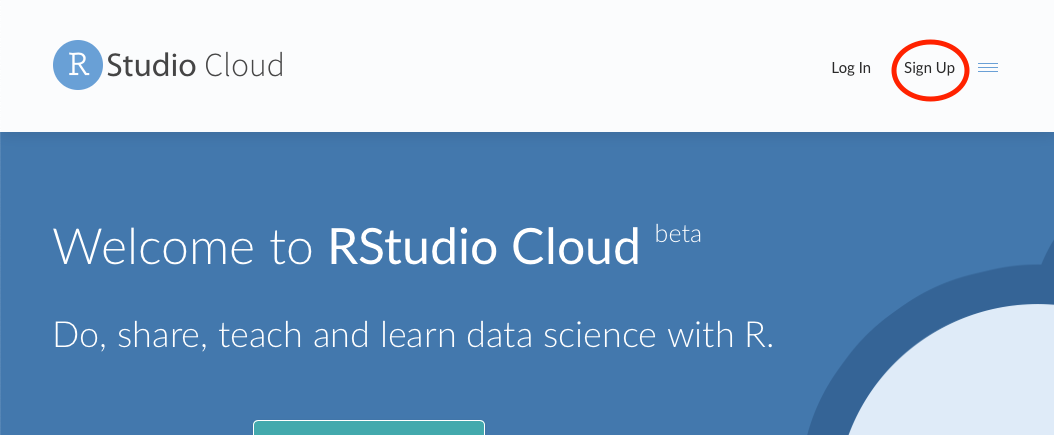
\includegraphics{img/signup.png}

Then join our shared RStudio cloud workspace with the link that I sent you in the email titled `Rstudio cloud shared workspace'.

\textbf{You MUST join our shared workspace.} I will be checking your work through this shared RStudio cloud workspace. Within this shared workspace, I will be able to see everyone's project, but you will only be able to see your project and my project.

Once you are in your Rstudio Cloud account\ldots{}

Expand the R studio cloud options by clicking on the 3 lines in the top left corner.

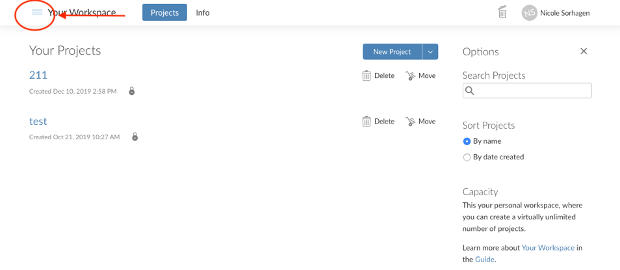
\includegraphics{img/Picture1.png}

Then select our course (which will be titled the name of course). If you cannot see this option -- then you have not been added to our shared workspace.

Once you are in the Class's shared workspace, open a new project. The new project button is on the top right.

Call this project your last name by clicking on the box that says `Untitled Project' and typing your last name.

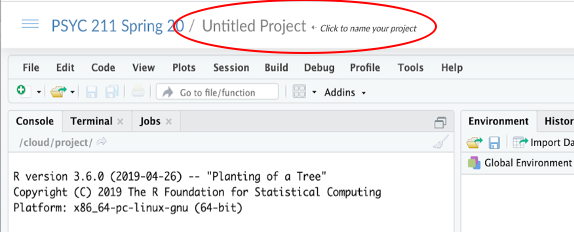
\includegraphics{img/Projname.png}

Congrats! You have successfully set up your project on our class RStudio Cloud workplace! You will use this project for all of your R work for the rest of the semester. Next let's learn a bit about the software environment and the R programming language.

\hypertarget{introduction}{%
\chapter{Introduction}\label{introduction}}

This chapter introduces the RStudio cloud environment and describes how to import data into the RStudio cloud.

R cannot handle typos and is case sensitive (`Gender' is not the same as `gender'). If your code will not run check for typos and caps.

Related to this point, do not be afraid to copy and paste with using R. I often copy and paste code and replace variable or dataset names as needed. (This is one of the few times in education where copy and paste is OK!)

\hypertarget{layout-of-rstudio}{%
\section{Layout of Rstudio}\label{layout-of-rstudio}}

Rstudio has four panes: the console panel, the script panel, the environment and history panel, and the files and plots panel. Each will be describe in turn next.

\hypertarget{console}{%
\subsection{Console}\label{console}}

The console panel of R studio is where you can type commands (or R code) and where you will see the output of commands.

In its most basic form, you can think of R as a fancy calculator.

For example: In the console type \texttt{2+2} and then press RETURN on your keyboard. The answer `4' will apear on the next line.

The \texttt{\textgreater{}} in the last line of the console means that the console is ready for a command (see red circle in the picture above).

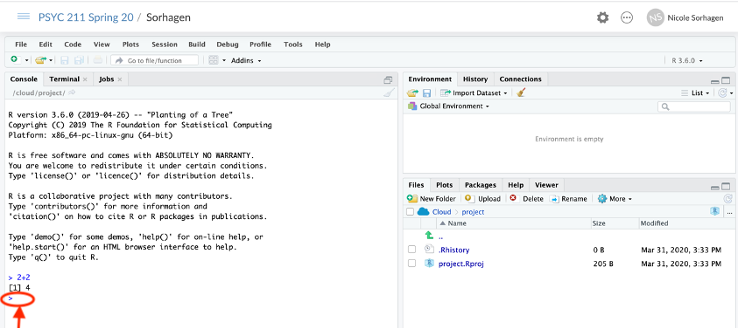
\includegraphics{img/twoplus.png}

If \texttt{\textgreater{}} is missing from the last line, it means that R is waiting for you to complete a command.

For example, type \texttt{1+} in the console and then hit enter.

The plus sign means the command is incomplete.

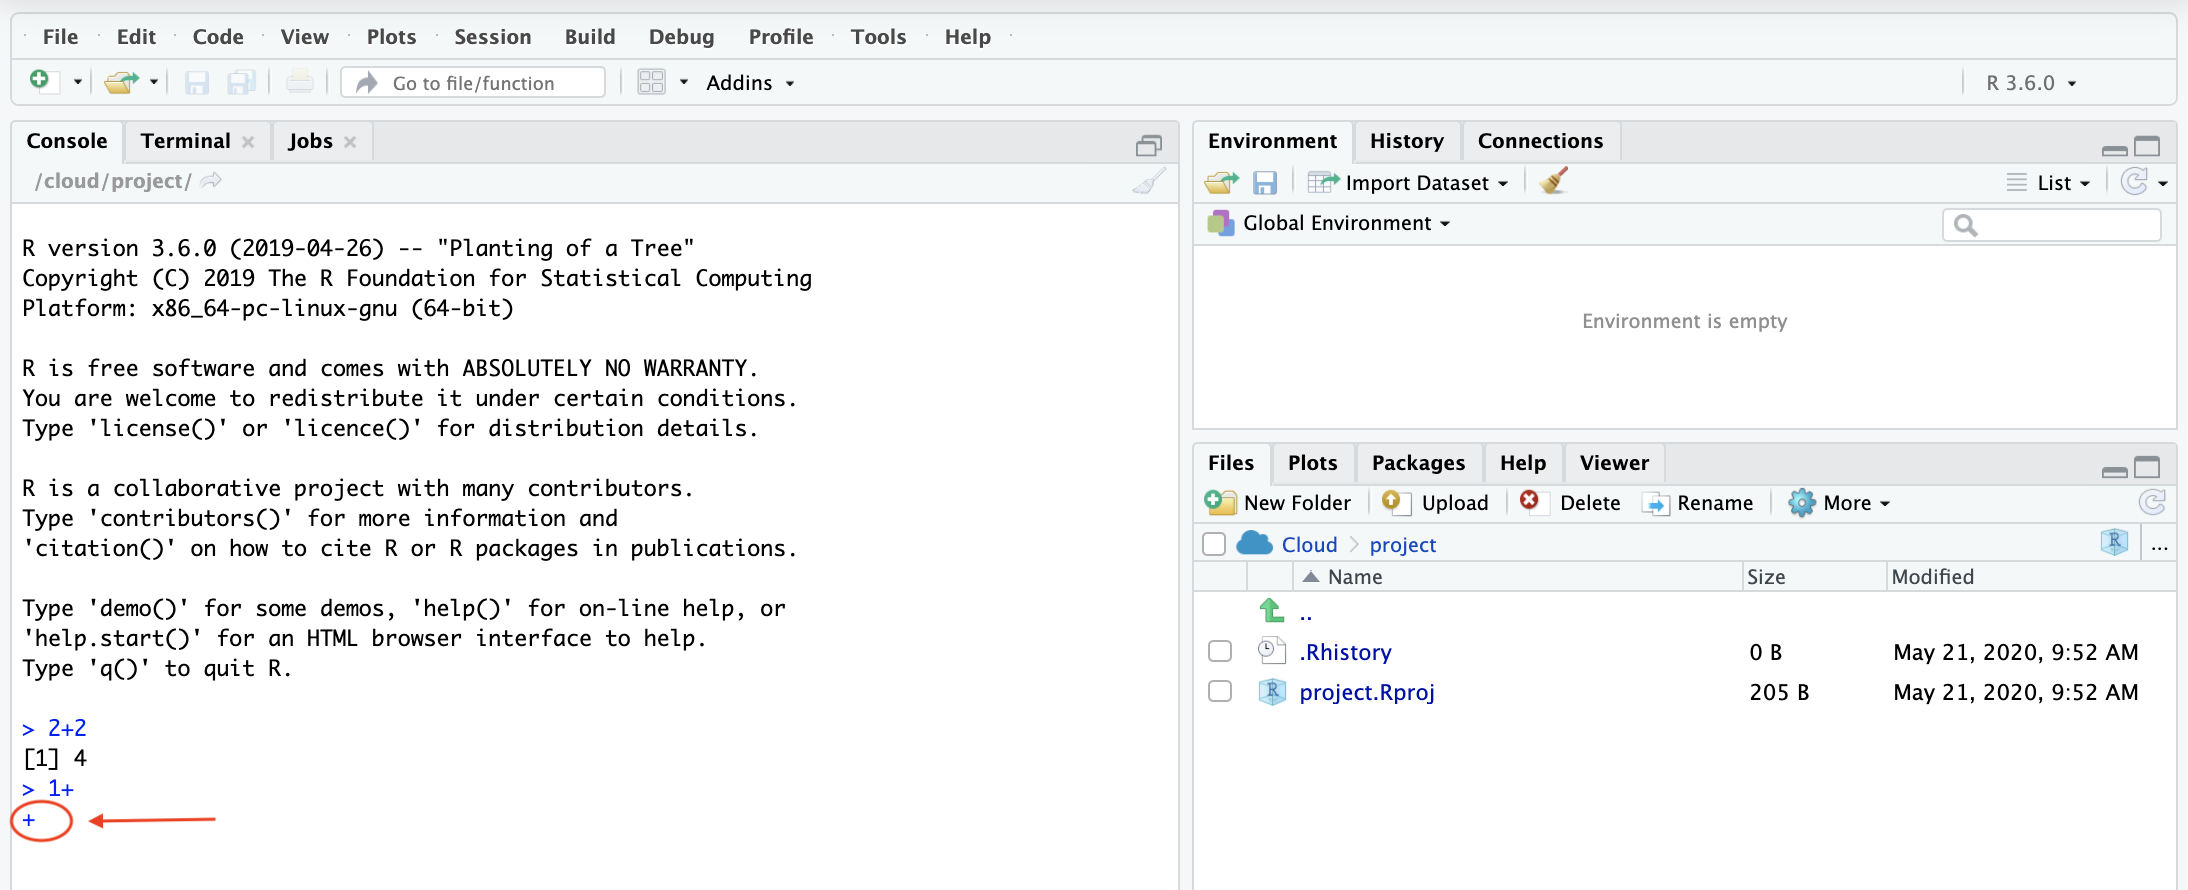
\includegraphics{img/waiting.png}

Push the \textbf{ESC} button on your keyboard to get back to the command prompt (\textgreater).

\hypertarget{script}{%
\subsection{Script}\label{script}}

One of the benefits of using R is that you can save a record of your work using scripts. Records of your work allow you to easily start and stop an assignment or research project. You can pick up where you left off whether it is 20 minutes later or 2 years later. These script files also let you share your data analysis with others -- from professors, to collaborators, to peer reviewers (ensure that your work is reproducible).

To create a new script, go to the top bar menu:

\textbf{FILE -\textgreater{} NEW FILE -\textgreater{} R SCRIPT}

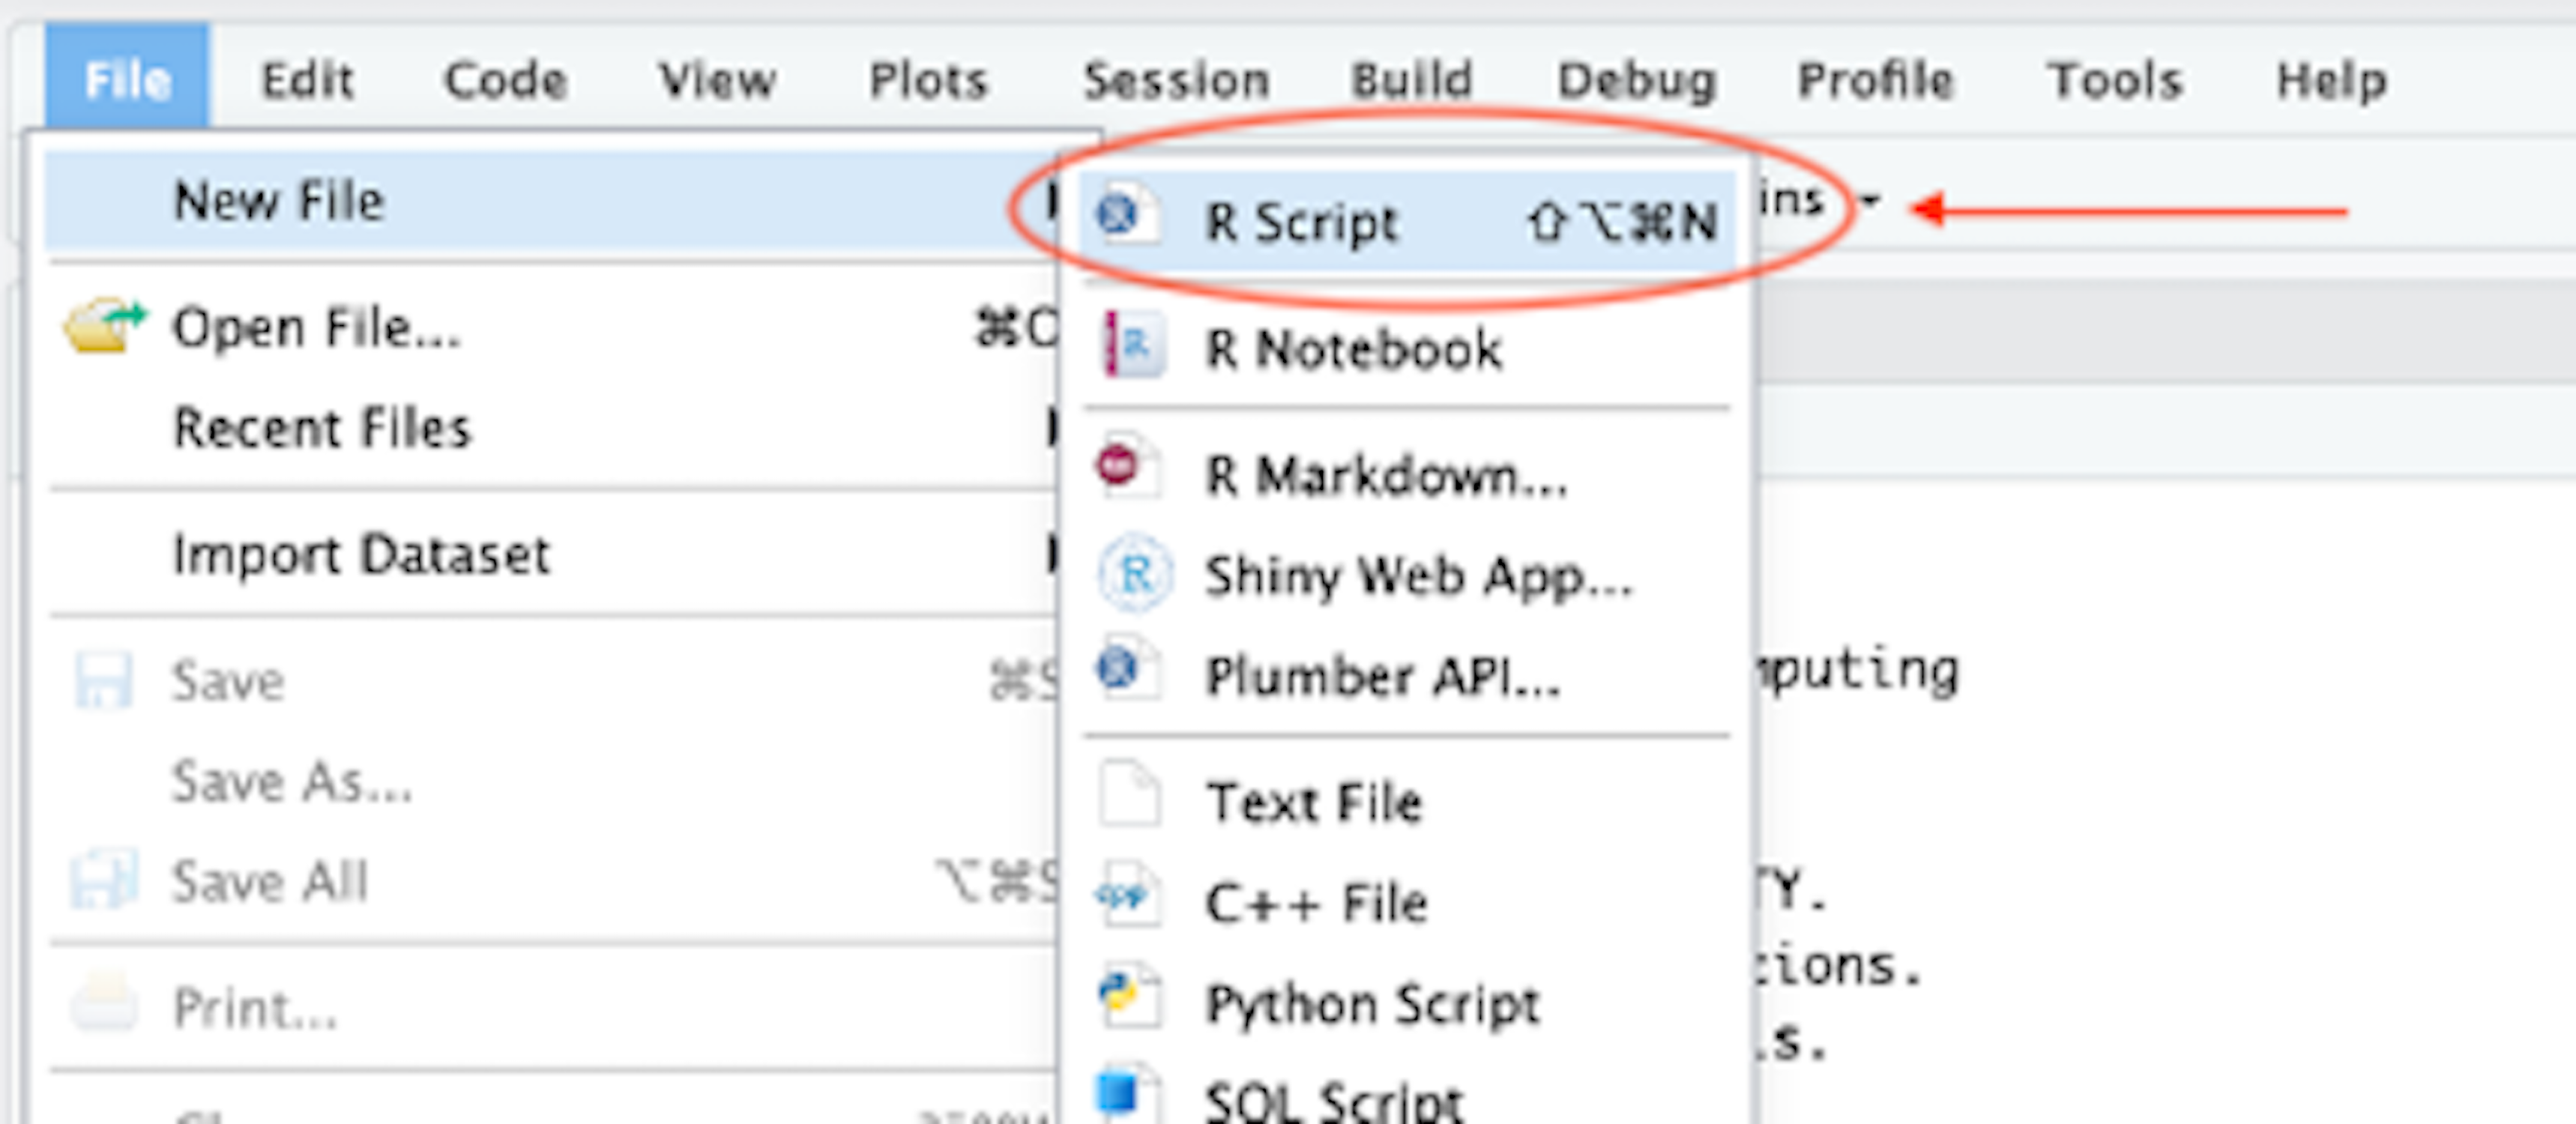
\includegraphics{img/newscript.png}

A new script will open in the top left of the RStudio platform.

\textbf{You should run code from scripts}

Scripts are similar to running command in the console (this is what you did in the last section).

For example, type \texttt{5+5} in the script panel.

In order to run command in a script you should click the run button while the cursor is in the code or the code is selected. Instead on clicking on the run button, you can also run the code by pressing the COMMAND and RETURN keys on your keyboard at the same time (the ALT and RETURN key on a pc).

After the code is run, the results will automatically appear the in console (see red arrow in the picture below).

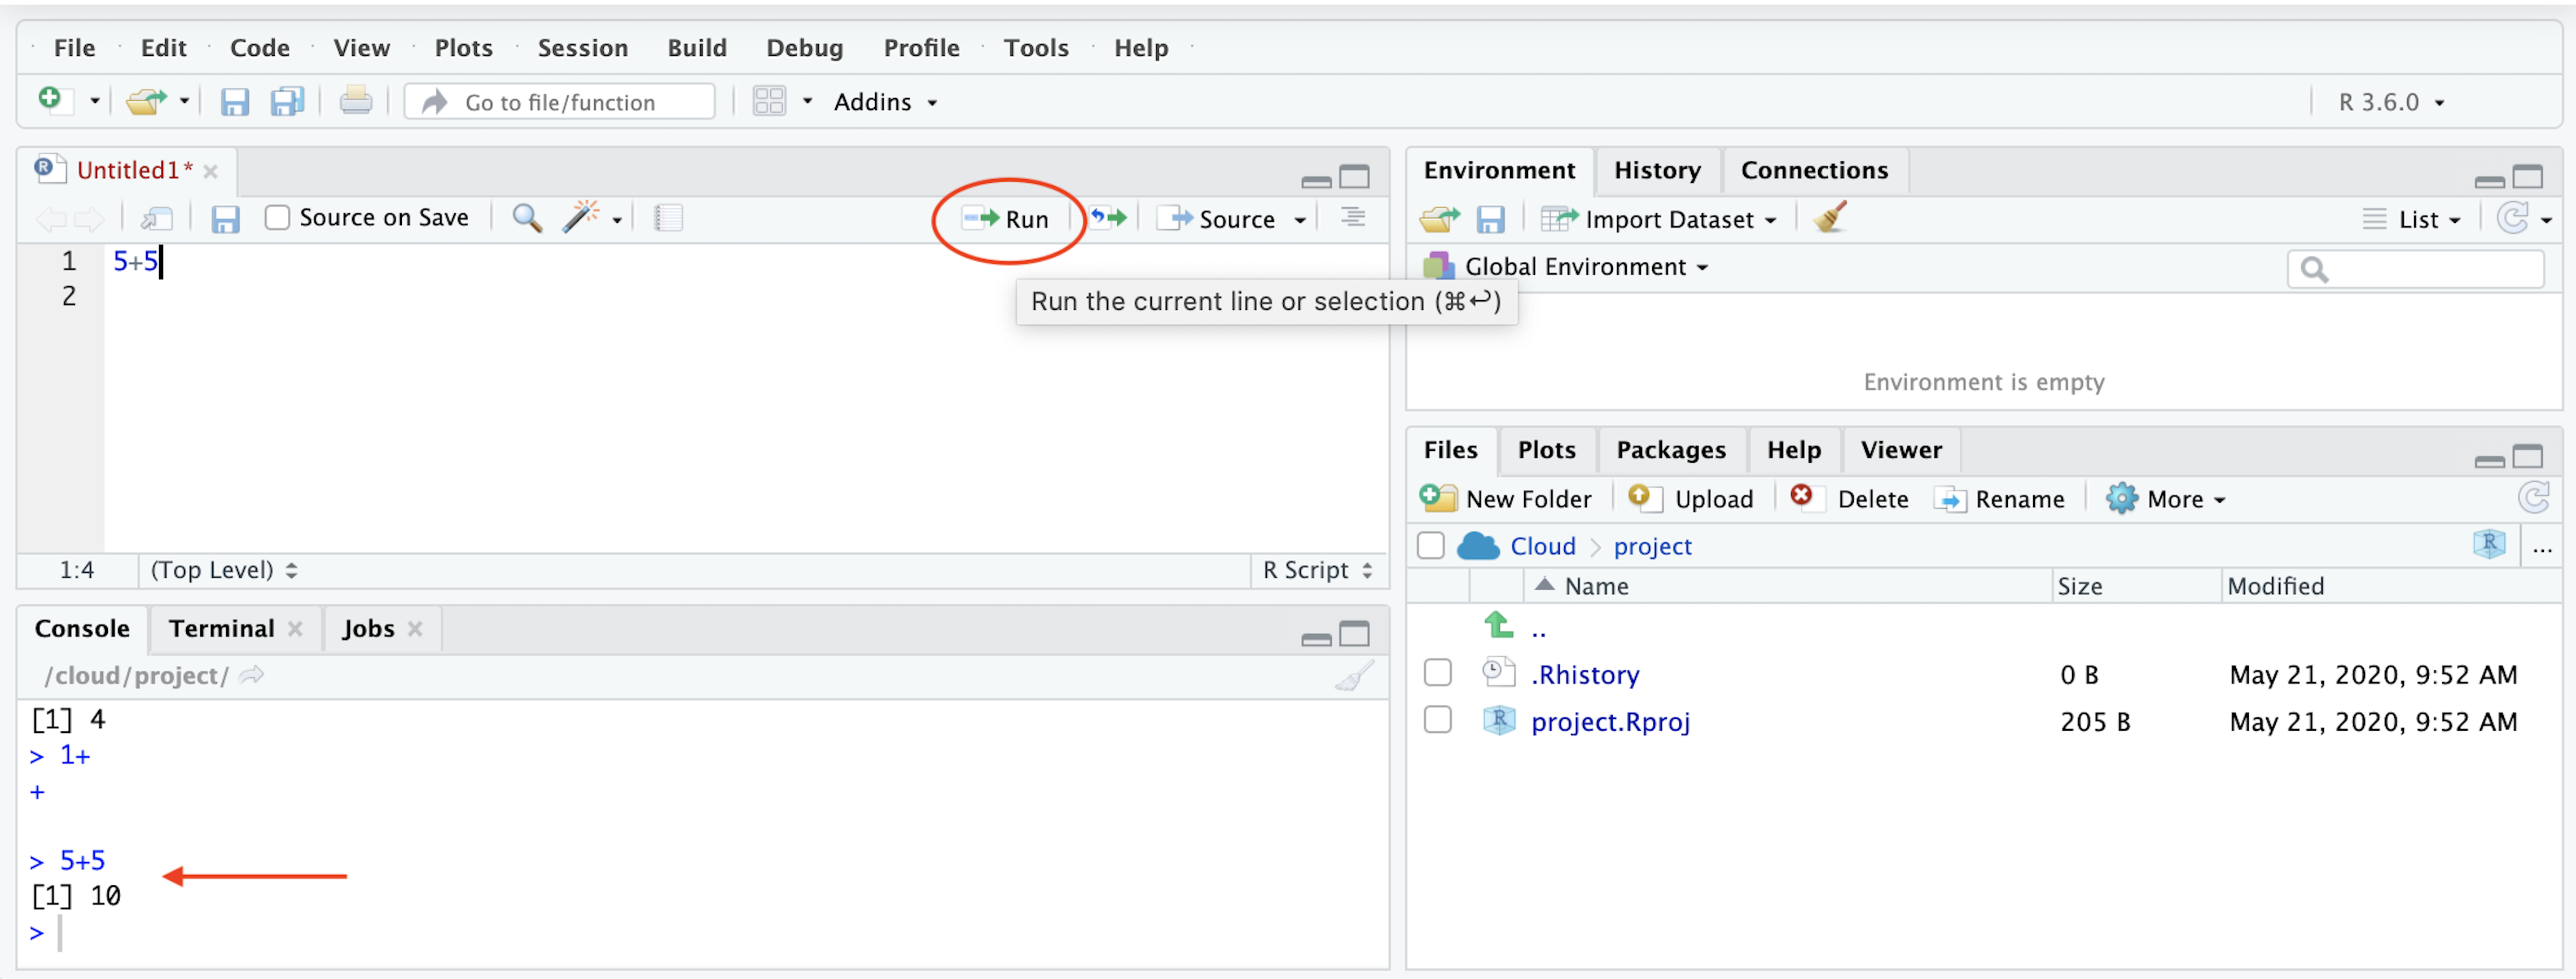
\includegraphics{img/script.png}

In order to use the script again you must \textbf{save} it.

From the drop-down menu select:

\textbf{FILE -\textgreater{} SAVE AS}

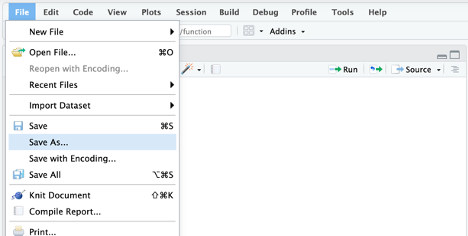
\includegraphics{img/savescript.png}

Type \textbf{lab 1} into the file name box. And then click the SAVE button.

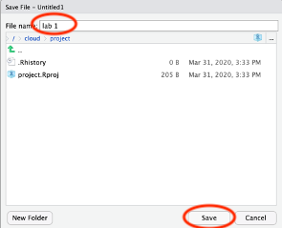
\includegraphics{img/savescript2.png}

Your file should now be listed in the files window in the bottom right.

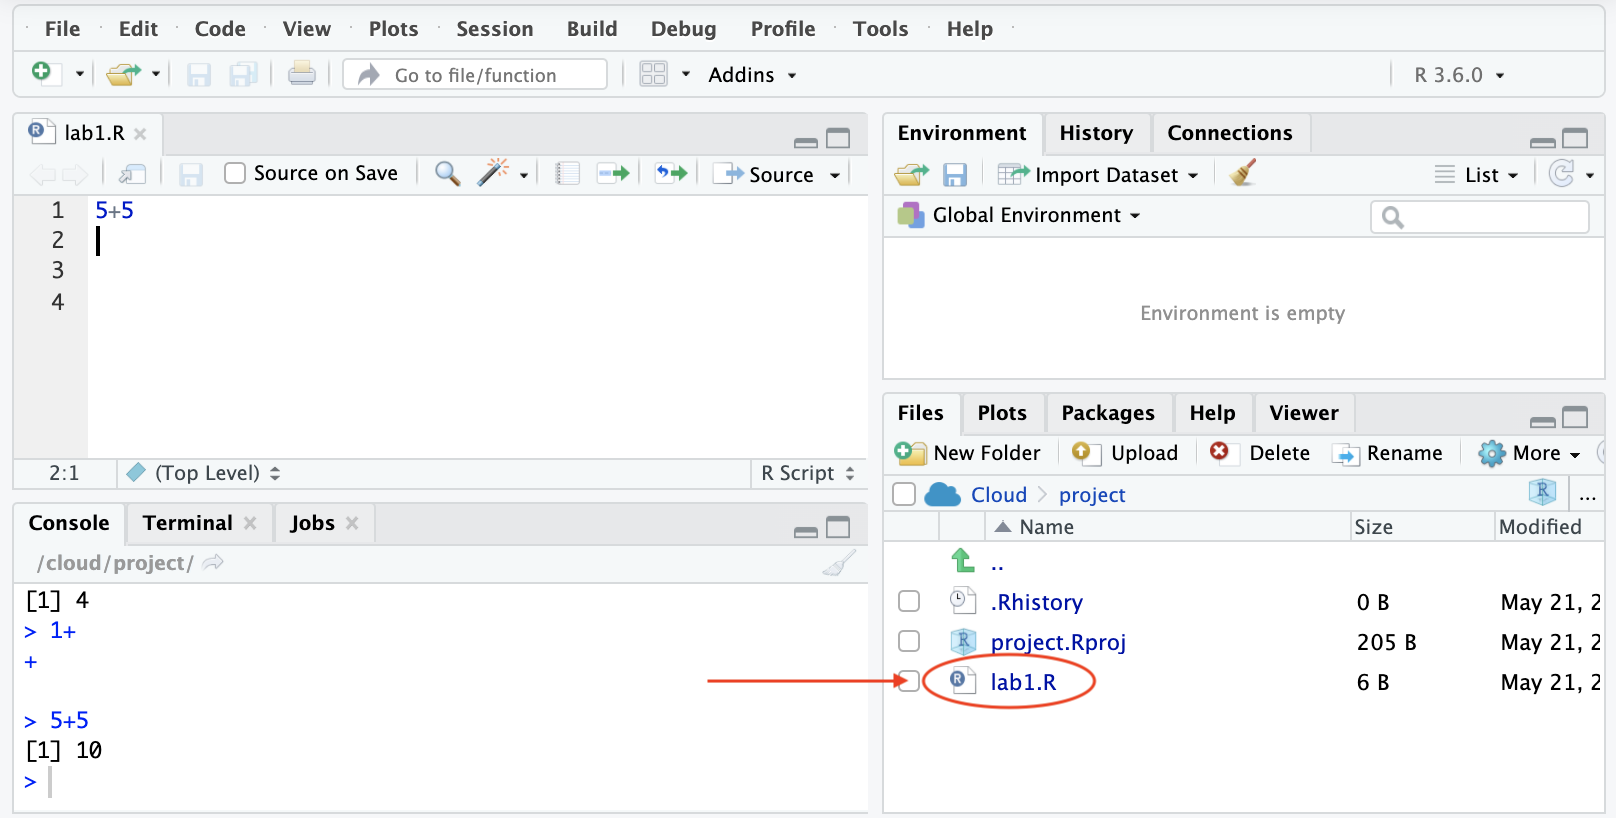
\includegraphics{img/savescript3.png}

\textbf{This script file is a record of your work and is how you will be graded for the `reproducing the assigned chapters' assignment. Make sure you saved this file and complete the rest of this lab in your `lab1' script.}

Within a script you should include comments to yourself and others using a \texttt{\#}. Anything with a \texttt{\#} in front of it will not run. \textbf{These comments and explanations are an important part of an R script.}

For example, type the following in to the script and then run it.

\texttt{\#r\ is\ like\ a\ calculator}

\texttt{2+2}

\texttt{\#Answer\ is\ 4}

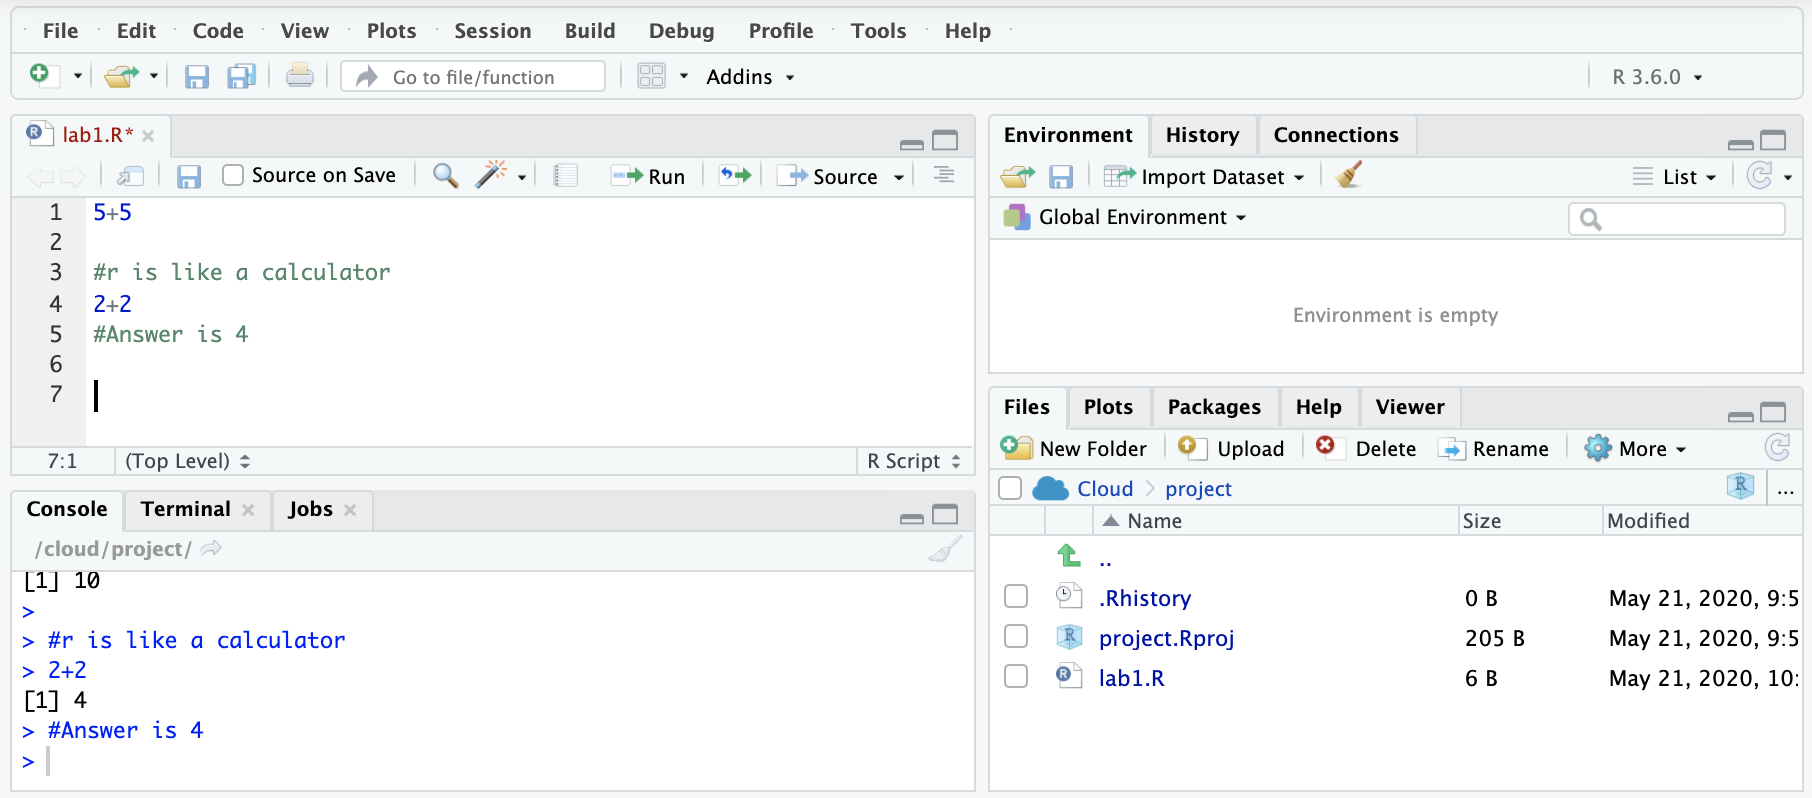
\includegraphics{img/comment.png}

Note that the comments appear green in the script.

You can make notes to me this way (if needed). For example:\\
\texttt{\#This\ will\ not\ run.\ Dr\ S,\ I\ need\ help}

I will leave comments to you this way. When I do, I will start my comment with my initials. For example:\\
\texttt{\#NS:\ try\ loading\ the\ tidyverse\ package\ first}

Scripts should be organized so that someone else can follow what you did.

\hypertarget{environment-and-history}{%
\subsection{Environment and history}\label{environment-and-history}}

In the top right corner of RStudio is the environment and history window. The \textbf{history tab} shows every line of code that has been run in the current session. I do not use this much.

The \textbf{environment tab} is where all active \textbf{objects} are listed. An object is something can hold information for later use. The information can be data, values, output, or functions. Normally my panel is set on this.

Objects are assigned using \texttt{\textless{}-}. Values on the right side of \texttt{\textless{}-} will be assigned to the object on the left side.

For example, let's tell R that the population mean of IQ scores is 100 and the population standard deviation is 15.

To do this use the following code:

\texttt{mu\ \textless{}-\ 100}

\texttt{sigma\ \textless{}-\ 15}

After you run these commands, the objects will now be listed in the environment panel in the top left.

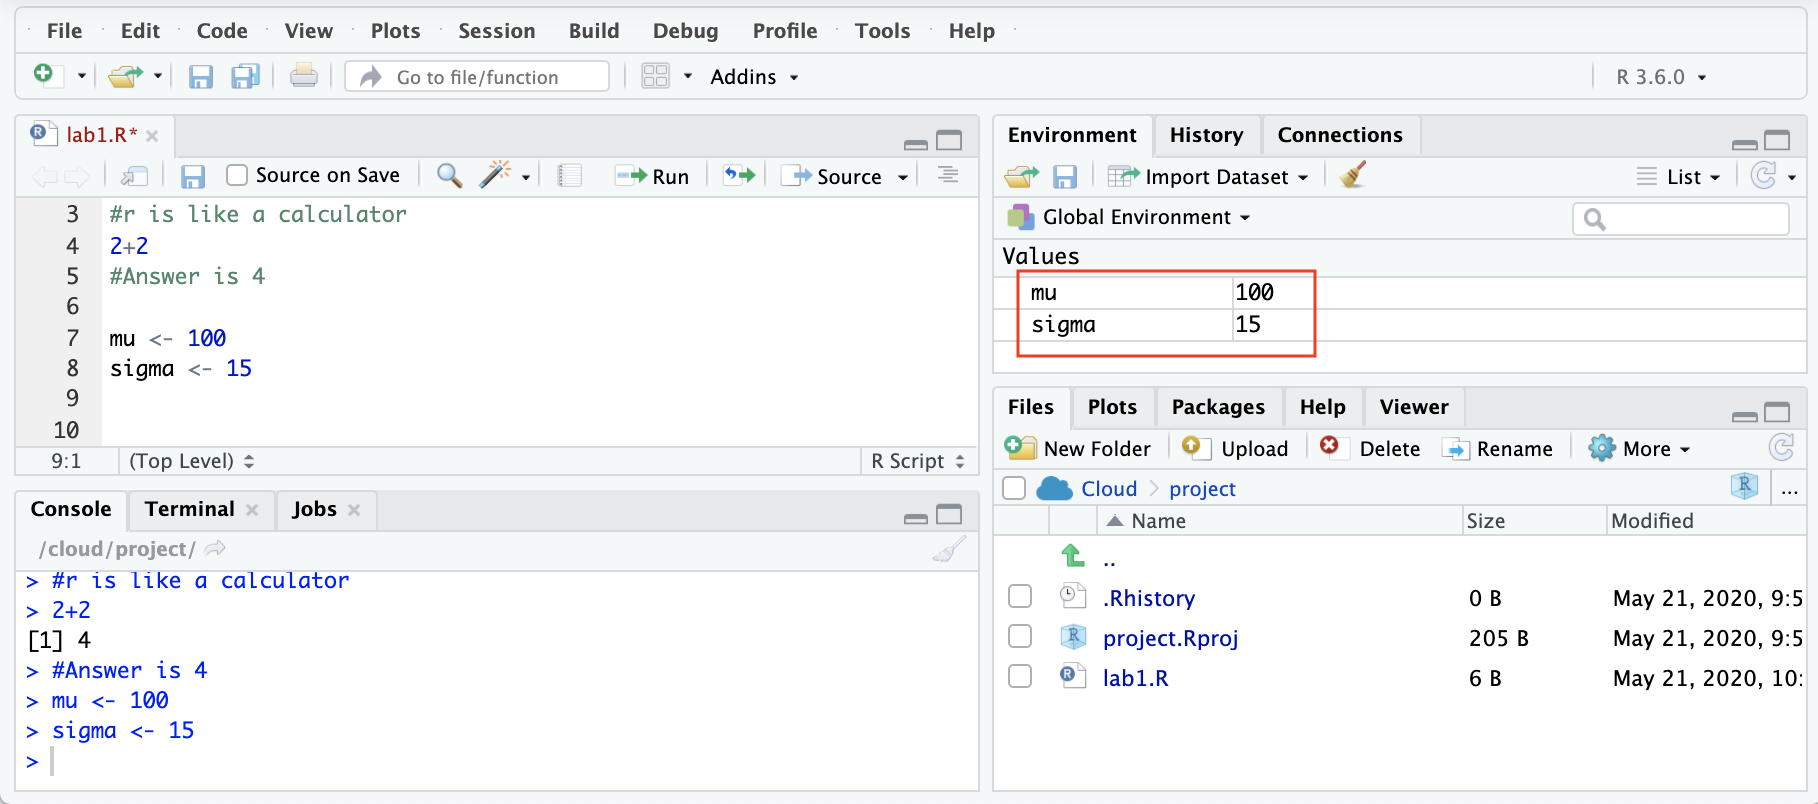
\includegraphics{img/object.png}

The shortcut for making \texttt{\textless{}-} is the ALT and -- key together. (or OPTION and -- on a mac)

\hypertarget{vectors}{%
\subsubsection{Vectors}\label{vectors}}

It is possible to store more than one number in an object. One way to do this is to use a \textbf{vector}. Assign a set of numbers a vector with the \textbf{combine} function: \texttt{c()}, by typing all of the numbers you want to store within the parentheses in a comma separated list.

For example, let's enter the IQ scores of students in a small class.

To do this use the following code:

\texttt{classIQ\ \textless{}-\ c(112,\ 115,\ 89,\ 95,\ 101)}

After you run this code, the classIQ vector should appear in the environment.

Here is a picture of what your screen should look like:

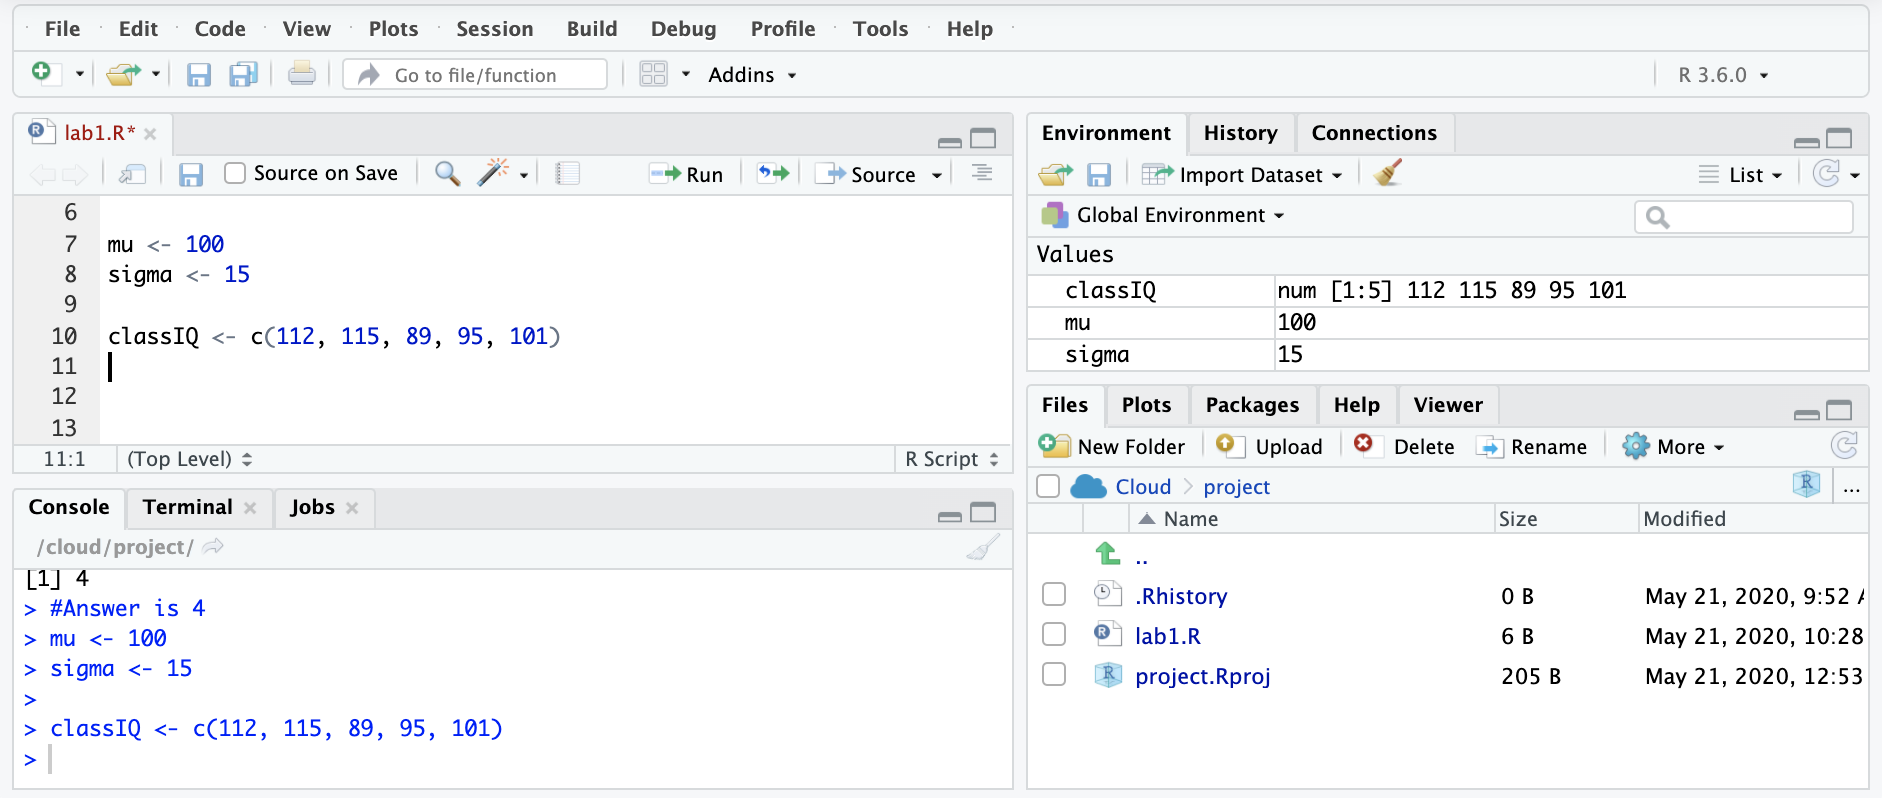
\includegraphics{img/vector.png}

Calculations with vectors apply to all data points.

For example, let's calculate the z-scores for each of the IQ scores.

To do this use the following code:

\texttt{\#get\ z-scores}

\texttt{(classIQ-mu)/sigma}

The results will appear in the console (See the red box in the picture below)

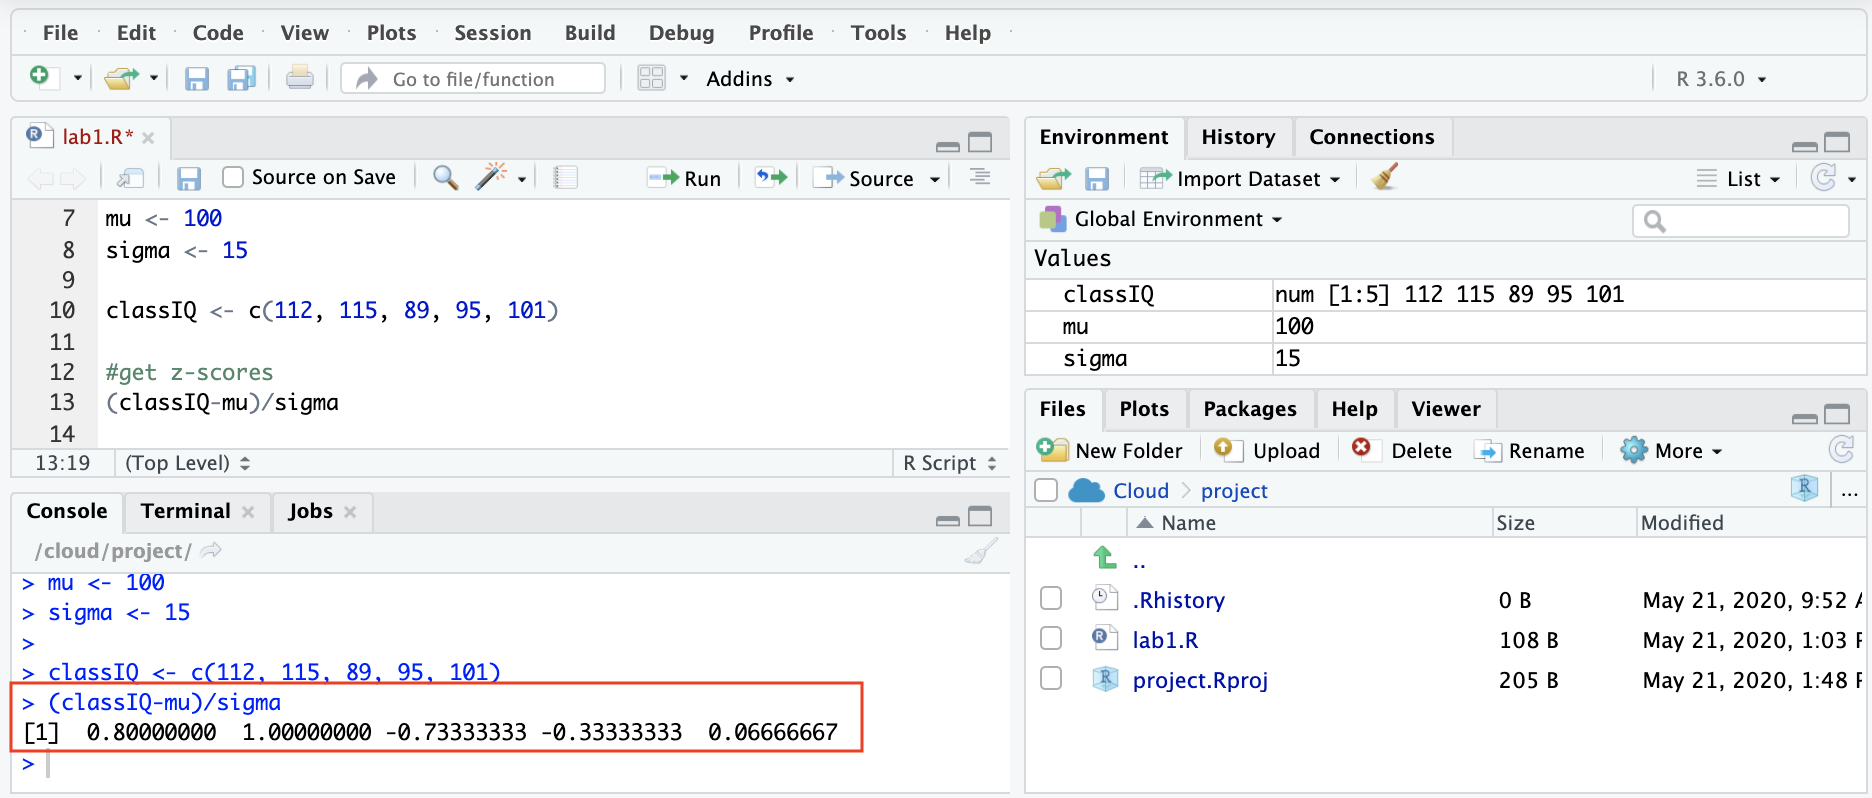
\includegraphics{img/zscores.png}

It is possible to save these answers as a vector using the \texttt{\textless{}-} function.

For example, let's save those zscores in a vector called zscores.

To do this use the following code:

\texttt{zscores\ \textless{}-\ (classIQ-mu)/sigma}

There should now be a vector in the environmnet called zscores.

Here is a picture so that you can check your progress:

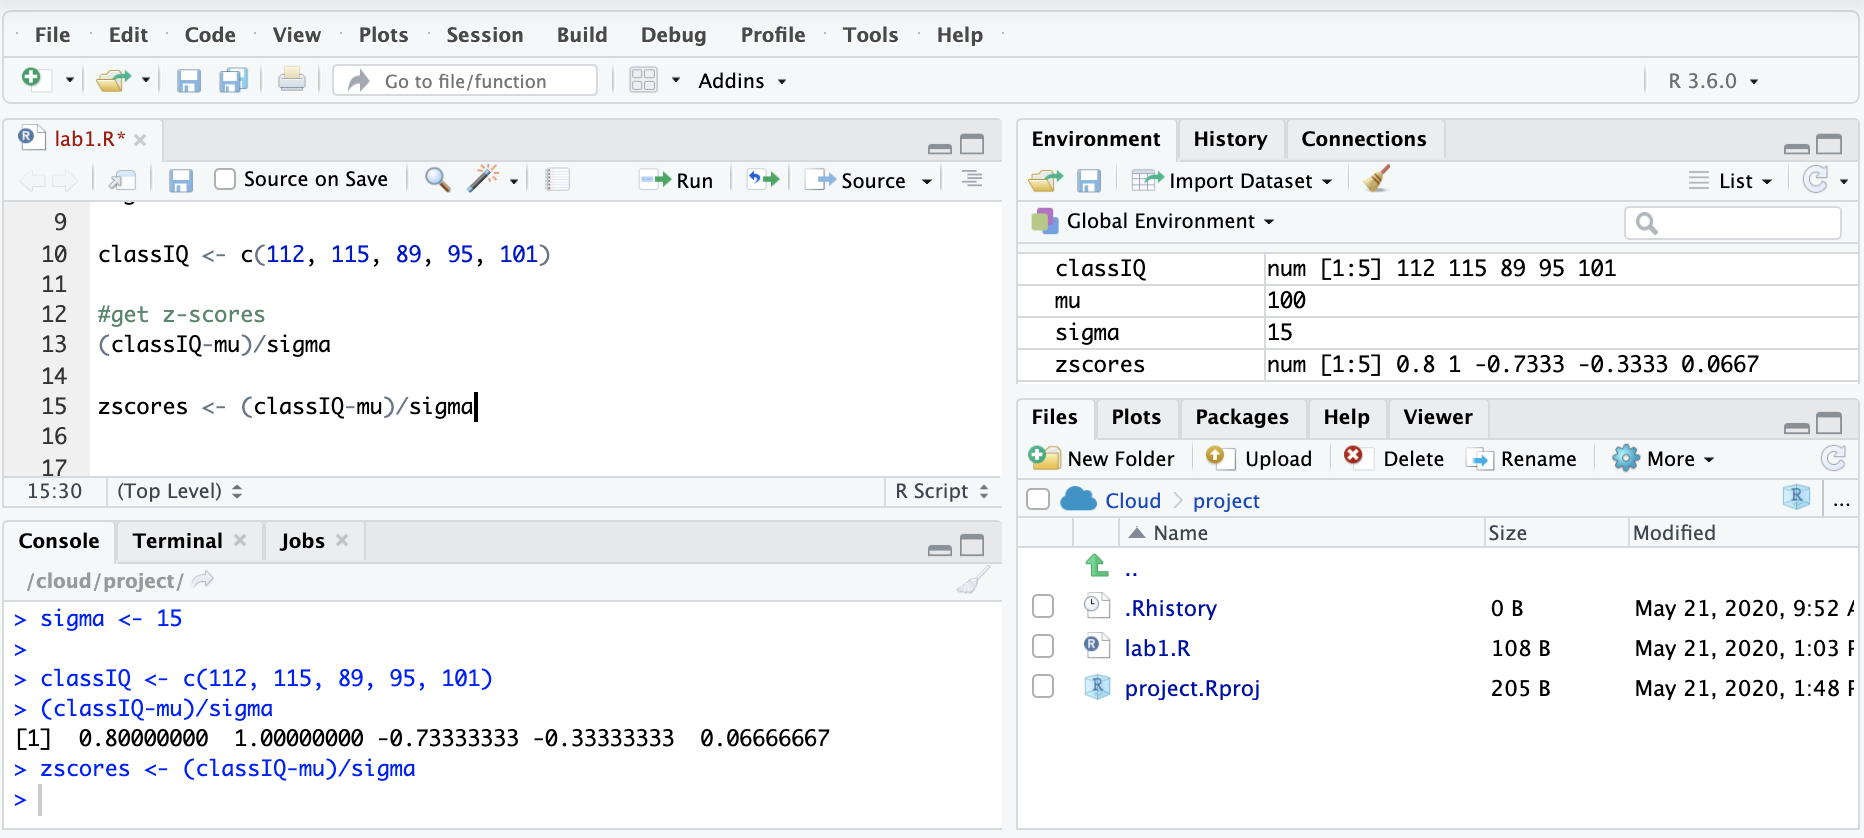
\includegraphics{img/zsaved.png}

\hypertarget{data-frames}{%
\subsubsection{Data frames}\label{data-frames}}

Right now the IQ scores and the z-scores are in separate objects. Variables often need to be in a single object in order to do some basic analyses. You can combine the classIQ and the zscores variable using the \textbf{data.frame} command.

To do this use the following code:

\texttt{iq\ \textless{}-\ data.frame(classIQ,\ zscores)}

\begin{itemize}
\tightlist
\item
  This command takes the form of DatasetName \textless- data.frame(Variable1, Variable2, etc)\\
\item
  The dataset name can be anything you want that you have not already used

  \begin{itemize}
  \tightlist
  \item
    the name must be one word (there cannot be spaces in the name)
  \end{itemize}
\end{itemize}

This object will be listed under data instead of values in the environment panel.

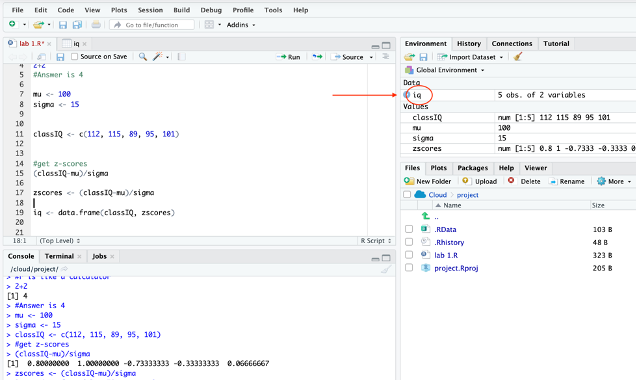
\includegraphics{img/dataframe.png}

Double-click on the word `iq' in the environment panel to look at the dataset that you just created (it is circled in red in the picture above).

A new tab will open with a spreadsheet view of the dataset. When you are done viewing the data, you can close it by click on the `x' next to the name iq.

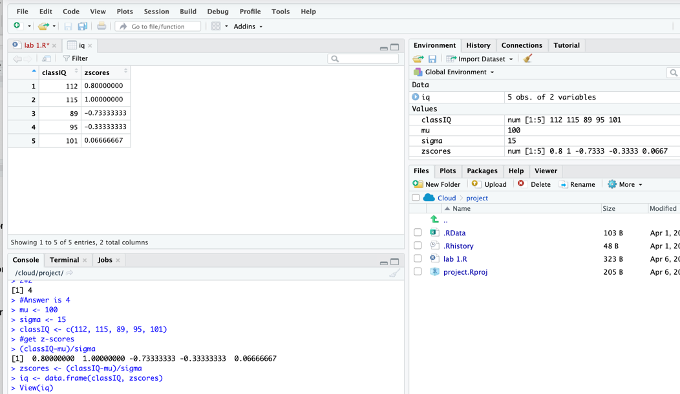
\includegraphics{img/dataframe2.png}

Note that after looking at the dataset this way, the command \texttt{view(iq)} appeared in the console. You can look at the dataset with the \textbf{view} command as well

When typing the code to create the data frame, you may have noticed that RStudio uses \textbf{predictive text}. This means that RStudio will suggest functions and objects as you type. You should take advantage of this feature!

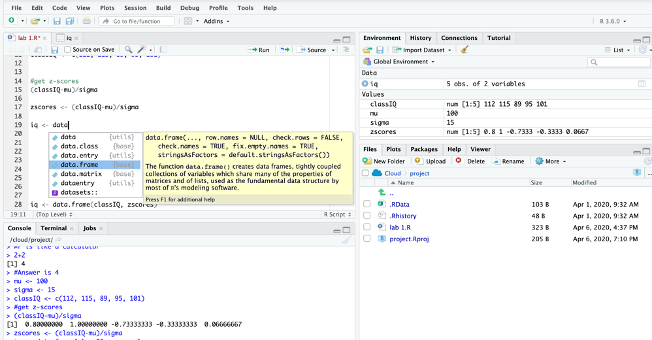
\includegraphics{img/autofill.png}

\hypertarget{importing-data-into-rstudio-cloud}{%
\section{Importing data into Rstudio cloud}\label{importing-data-into-rstudio-cloud}}

In the last section you learned how to assign data to a \textbf{vector} using the \textbf{combine} function.

Another way to assign data to an object is by first entering the data into a spreadsheet (like google sheets or excel) and then import the data into RStudio. This will be our preferred method.

\textbf{First download the exam2.csv file from d2l.}

This file contains data on the exam 2 scores from a previous class of mine. It also has some made up data on students' studying, eating, and drinking behaviors before the exam.\\
Make sure the file remains a .cvs file after you download it. If you open it in excel, excel might change the file to an .xls file.

When using RStudio in the cloud, you will first need to uplaod the data into your project and then import it into the global environment.

\hypertarget{upload-the-data-into-rstudio-cloud}{%
\subsection{Upload the data into Rstudio Cloud}\label{upload-the-data-into-rstudio-cloud}}

Then select the UPLOAD button in the files window.

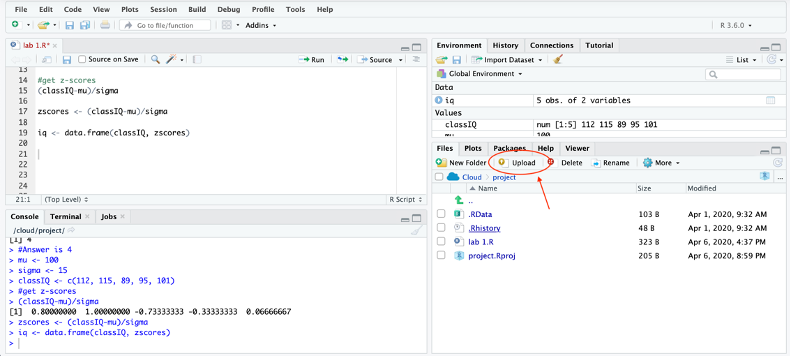
\includegraphics{img/upload.png}

In the Upload Files window, click the CHOOSE FILE button and then navigate to the exam2.csv file on your computer. Then click the OK button.

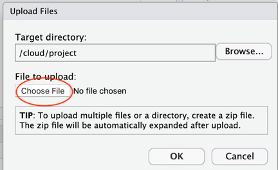
\includegraphics{img/choosefile.png}

The data file should now be listed in the files section of RStudio.

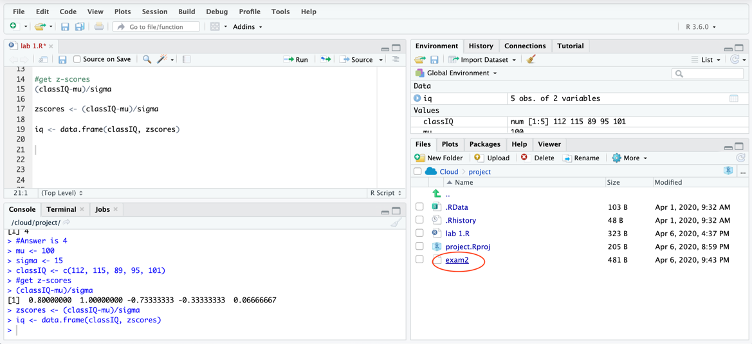
\includegraphics{img/filelist.png}

\hypertarget{import-data}{%
\subsection{Import data}\label{import-data}}

Then you need to import the data into the environment (i.e.~assign the data to an object). This can be done through using point and click options or with code.

\hypertarget{point-and-click}{%
\subsubsection{Point and click}\label{point-and-click}}

First click on the \textbf{IMPORT DATASET} button in the environment panel.

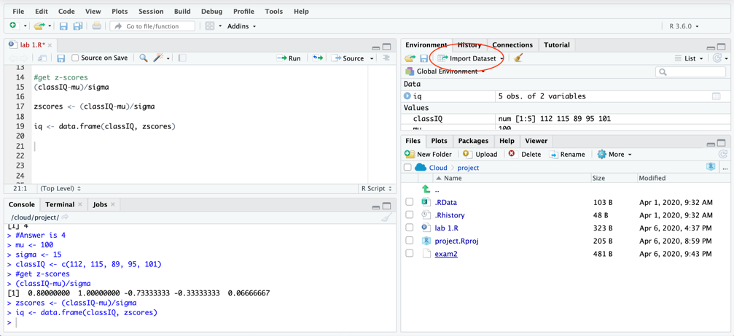
\includegraphics{img/import.png}

Then select the \textbf{`FROM TEXT (READR)'}

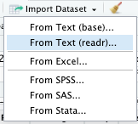
\includegraphics{img/readrbox.png}

The first time you select this -- the following window will appear asking if you would like to install the readr package. Select YES. I will introduce packages in the next section.

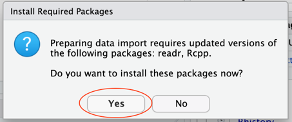
\includegraphics{img/installreadrbox.png}

After you select yes, R will begin downloading the package. This can take a few minutes and will look something like this:

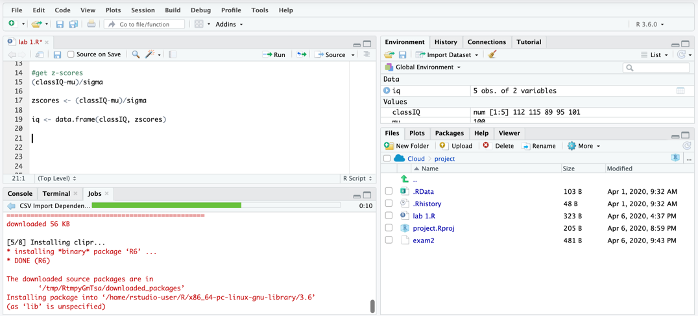
\includegraphics{img/installreadr.png}

It is important to be \emph{patient} here and let the package download completely before you move on to the next step.

When the download is complete, your screen should look like this:

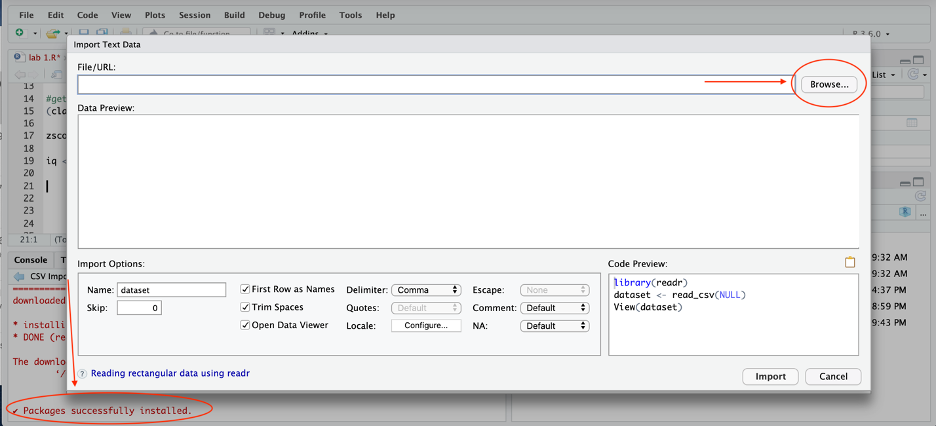
\includegraphics{img/importwindow.png}

Note that you can see that the package was successfully installed in the console in the bottom left. The next time you use readr to import data -- you will not have to download the package first.

Next select the BROWSE button in the top left corner of the import data window.

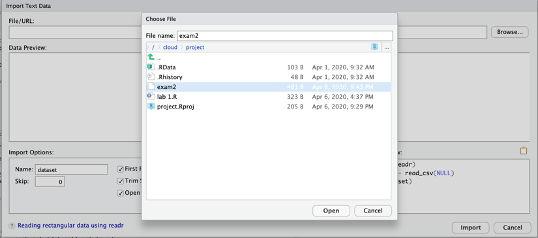
\includegraphics{img/importbrowse.png}

In the choose file window, select `exam2'. And then select OPEN.

The next window should look like this:

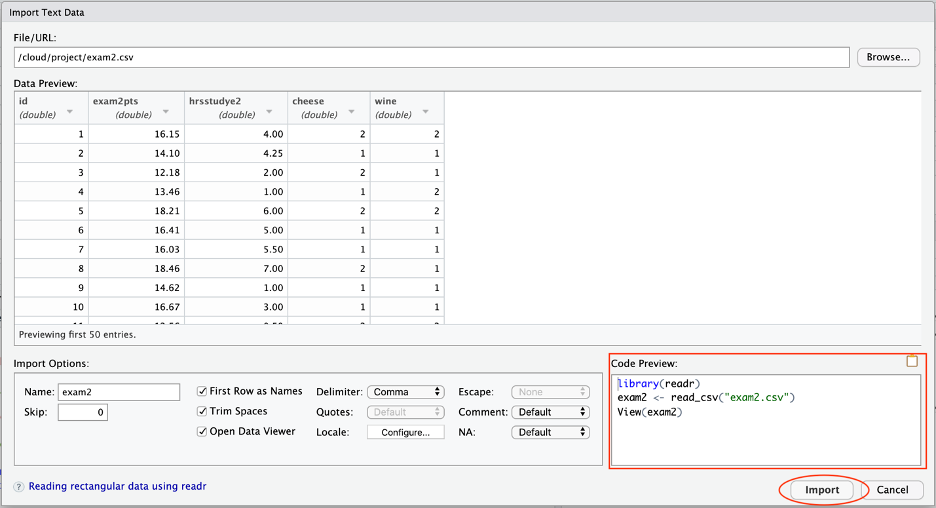
\includegraphics{img/importwindow2.png}

From here you should click the IMPORT button.

But first note the \textbf{Code Preview} box. This is the code you could use to import data (instead of clicking through all these windows). It's a good idea to copy this code before you click the import button and then paste it into your script for your records and in case you need to assign the file to an object again (because it is faster with code).

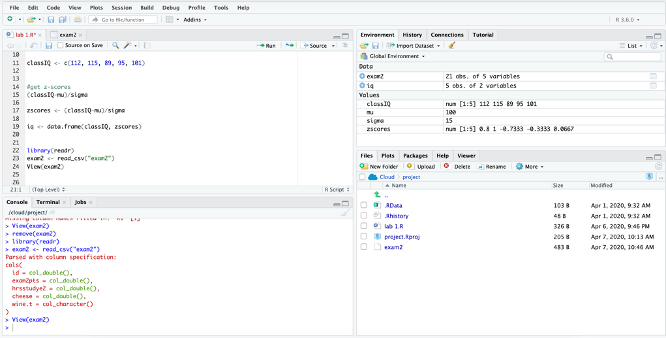
\includegraphics{img/importcomplete.png}

\hypertarget{code}{%
\subsubsection{Code}\label{code}}

Alternatively you could have typed the code that you copy and pasted (and not gone through all of the point and click windows).

\texttt{Library(readr)}\\
\texttt{exam2\ \textless{}-\ read\_cvs("exam2.csv")}

\begin{itemize}
\tightlist
\item
  This command takes the form of DatasetName \textless- read\_cvs(``FILENAME.csv'')\\
\item
  The dataset name can be anything that you have not already used

  \begin{itemize}
  \tightlist
  \item
    the name must be one word (there cannot be spaces in the name)\\
  \end{itemize}
\item
  If you have not installed the readr package, you will have to so first (see the packages chapter for more information)
\end{itemize}

\hypertarget{view-data}{%
\subsubsection{View data}\label{view-data}}

Double click on the word exam2 in the environment panel to look at the dataset.

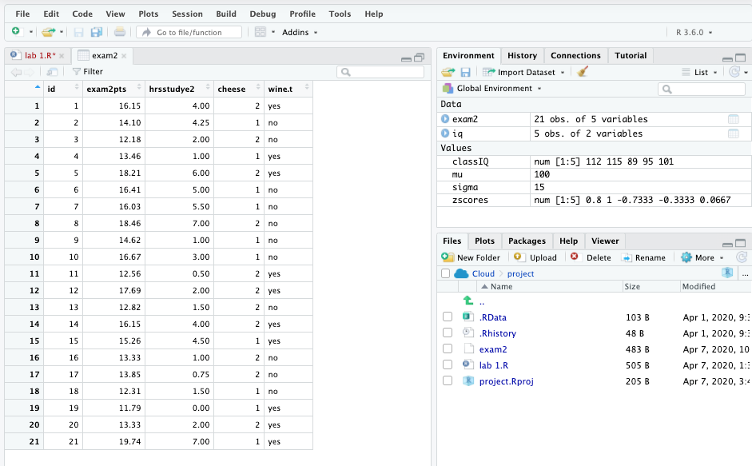
\includegraphics{img/view.png}

Each column is a different variable. Each row is a different participant (in this example a student).\\
- The first column is an arbitrary student ID number -- so that the students' identity is protected.\\
- The second column is exam points earned by the students out of 20 (this is real data from a Fall 2019 class).\\
- The third column is the number of hours the students studied for the exam (this is made up data).\\
- The fourth column is whether or not students ate cheese the night before the exam (1 = no; 2 = yes\ldots{} also made up data).\\
- The last column is data on whether or not students drank wine the night before the exam (1 = no; 2 = yes\ldots{} also made up data).

\hypertarget{packages}{%
\chapter{Packages}\label{packages}}

\textbf{NOTE:} Please open a new script and call it lab 2 (or week 2) for the replication of this chapter and the picturing data chapter assignment.

\textbf{Base R} refers to the functions that automatically come with R. But many people build on top of Base R to make R better. The way they do this is through \textbf{packages}, which contain new R functions. There are thousands of packages available that can do fancy things like quickly compute descriptive statistics and create APA style tables (and much much more).

The first time you use a package, you need to install it. Once a package is installed, you will need to tell R that you want to use it by loading it. You will need to load any packages you want to use each time you open the R program. (I am not exactly sure how this works in the RStudio cloud because it does not seem to shut down when you close out of the RStudio cloud website. See the Restarting R section below for a work around.)

That is, you only have to install a package once. You will have to load a package every time you want to use it.

\hypertarget{installing-packages}{%
\section{Installing packages}\label{installing-packages}}

The first time you use a package, you need to install it. We actually did this once already while importing data! This time let's learn more about the process.

In RStudio, packages can be installed through point and click (GUI) or with code.

\hypertarget{installing-packages-using-point-and-click-gui}{%
\subsection{Installing packages using point and click (GUI)}\label{installing-packages-using-point-and-click-gui}}

Let's first install a package called \textbf{Tidyverse}. Tidyverse was created by Hadley Wickham and his team with the aim of making various aspects of data analysis in R easier. It is actually collection of packages that include a lot of functions (e.g., subsetting, transforming, visualizing) that many people think of as essential for data analysis. (See the tidyverse website for additional information: \url{https://www.tidyverse.org}).

To install a package with GUI go to the top bar menu:

TOOLS -\textgreater{} INSTALL PACKAGES

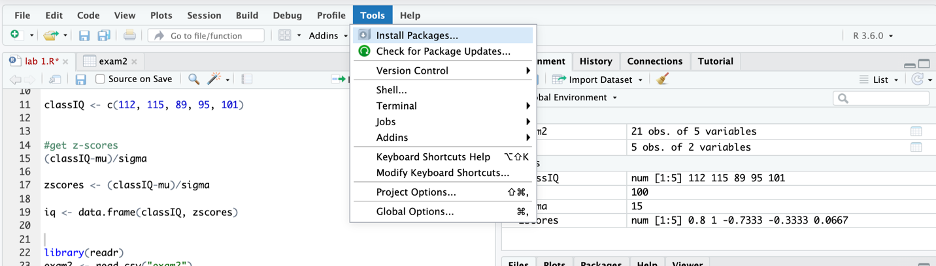
\includegraphics{img/instpacktools.png}

In the install packages window, type the name of the package you would like to install. For example, type \texttt{tidyverse} in the packages box.

Then click INSTALL.

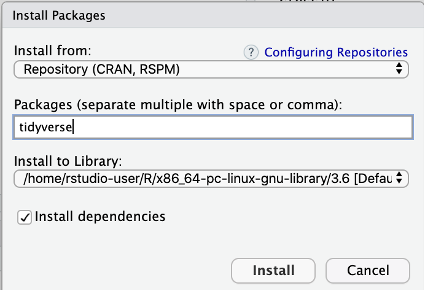
\includegraphics{img/instpackguitidy.png}

Again, installing a package can be a little slow on the RStudio cloud. Please be patient (maybe this is a good time to stretch your legs, refill your beverage, let the dog out, etc.)

Your screen should look like this when it is starting to install:

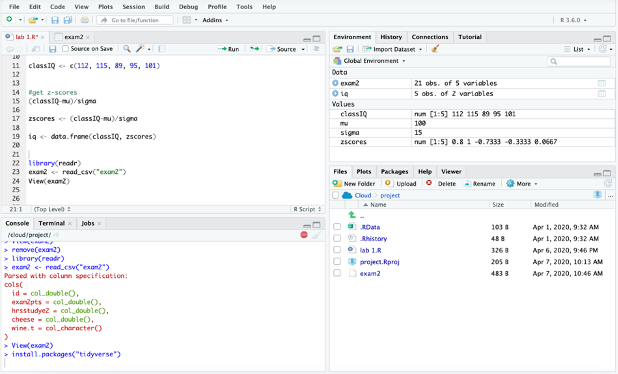
\includegraphics{img/instload1.png}

It should look like this when it is in the process of installing:

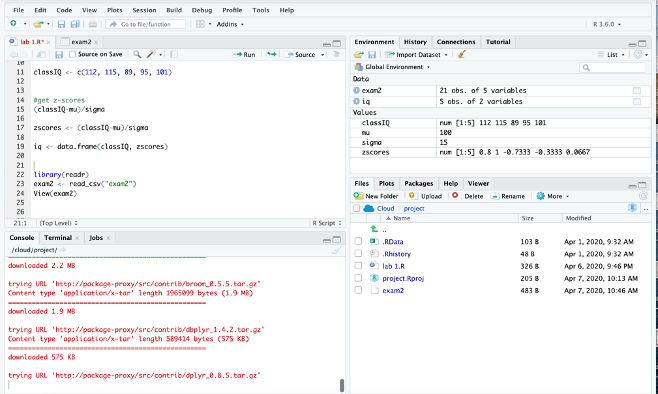
\includegraphics{img/instload2.png}

And then this when the installation is complete:

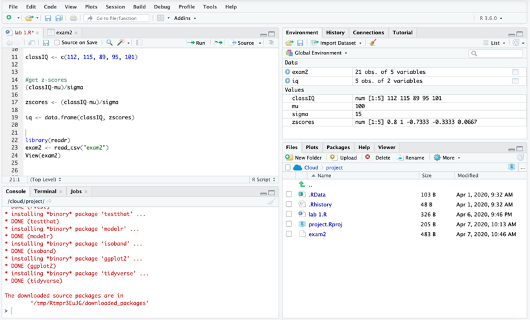
\includegraphics{img/instload3.png}

Do not proceed until the console says the package has been installed.

\hypertarget{installing-packages-using-code}{%
\subsection{Installing packages using code}\label{installing-packages-using-code}}

You can also install a package using this code:\\
\texttt{install.packages()}

To install tidyverse, for example, you would use this code:\\
\texttt{install.packages("tidyverse")}~\\
- Note that the word tidyverse is in quotes

But do not run this code -- as you have already installed it with GUI.

Instead, let's install a package called psych using the \texttt{install.packages} command. The \textbf{psych package} is a package for personality, psychometric, and psychological research. It has been developed at Northwestern University (maintained by William Revelle) to include useful functions for personality and psychological research.

To install this package, use following command:\\
\texttt{install.packages("psych")}

Your screen should look like this when the package is completely installed:\\
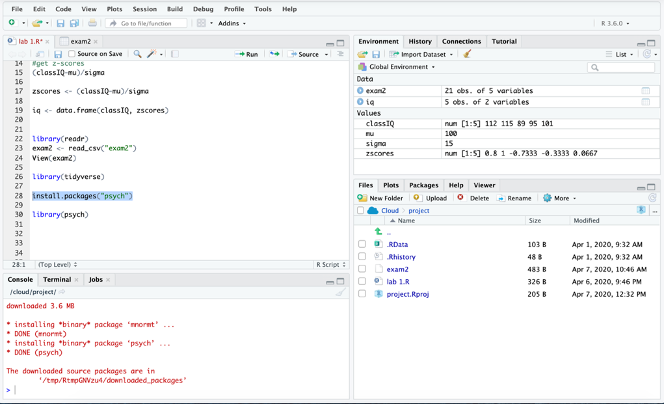
\includegraphics{img/instpsyc.png}

Remember that installing packages is the first step to using them and they only have to be installed once.

Next let's learn how to load packages, so that you can use thier functions.

\hypertarget{loading-packages}{%
\section{Loading Packages}\label{loading-packages}}

Installing a package is only the first step.

\textbf{In order to use a package, it must be loaded first.}

Packages can only be loaded with code. Packages need to be loaded every time you open the RStudio program. Most people's R scripts begin with the code that load packages.

When you have the Rstudio program installed on your computer this is straight forward (either the program is open or closed). This is less clear with Rstudio cloud because it does not seem to always shut down when you close the web browser site. (Please see the section on restarting Rstudio in the misc section below for a work around.)

The command to load a package is:\\
\texttt{library()}

For example, load the tidyverse package with this:\\
\texttt{library(tidyverse)}

After you run this code, your screen should look like this:

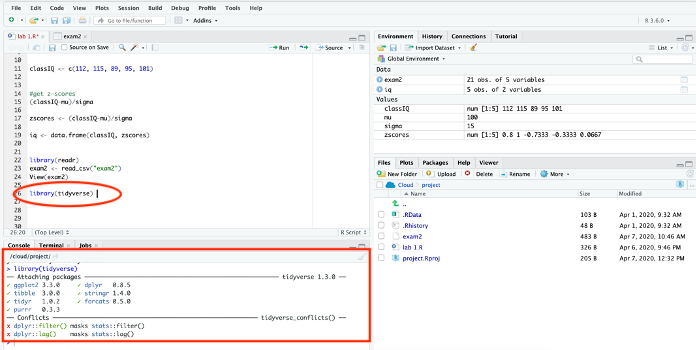
\includegraphics{img/loadtidy.png}

The console shows that the Tidyverse package has been loaded (don't worry about the conflicts for now).

Next let's load the psych package using this command:\\
\texttt{library(psych)}

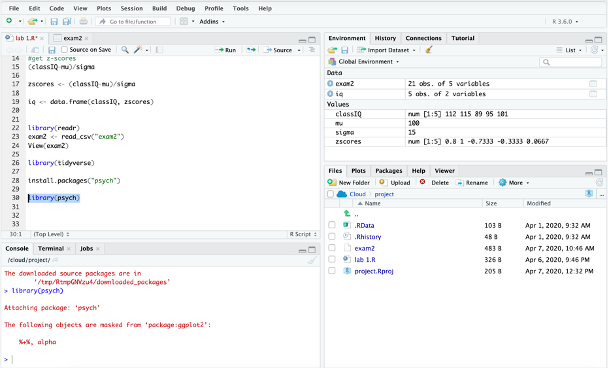
\includegraphics{img/loadpsyc.png}
Again, don't worry about the warning about masked functions for now.

\hypertarget{misc}{%
\section{Misc}\label{misc}}

You can get additional information using the \texttt{help()} function and \texttt{?} help operator in R. They both provide access to documentation pages for all functions and packages.

For example, use the following code to get more information about Tidyverse:\\
\texttt{?tidyverse}

Or this command to get more information about Psych:

\texttt{help(psych)}

\hypertarget{restarting-r}{%
\subsection{Restarting R}\label{restarting-r}}

Because it is unclear whether Rstudio completely turns off when you close the website, you could restart the R session to simulate the act of closing and reopening the Rstudio program (like you could if it were installed on your computer).

To do this, in the drop down menu go to:

SESSION -\textgreater{} RESTART R

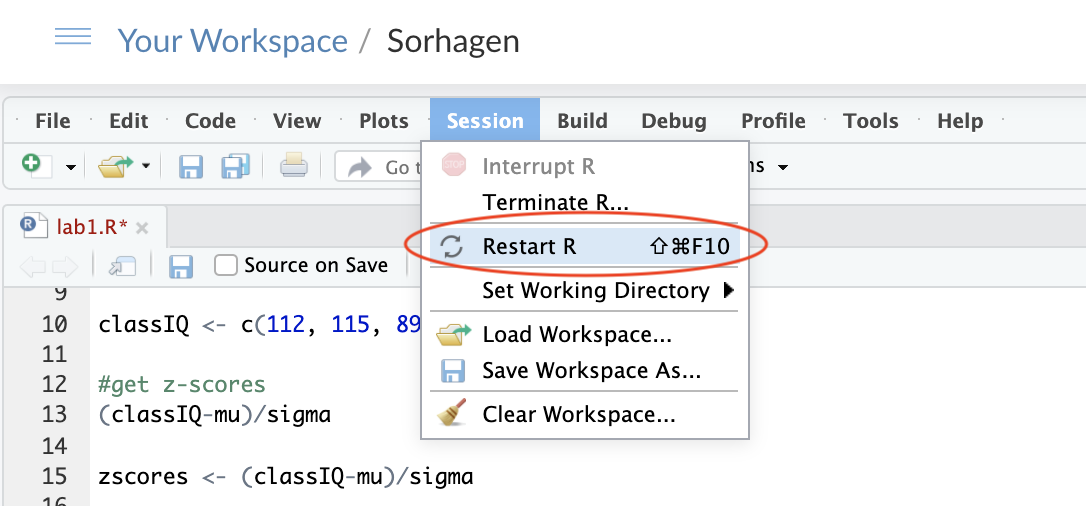
\includegraphics{img/restart.png}

When you restart the R session, everything in the script, environment, console, and files will remain.

All packages that were loaded will be cleared, so you will have to reload them if you want to use them.

If something is not working like it is suppose to (and you have checked for type-os), try restarting the R session. It could be that the functions of one package conflict or mask the functions of another package.

\hypertarget{picturing-data}{%
\chapter{Picturing Data}\label{picturing-data}}

``The simple graph has brought more information to the data analyst's mind than any other device.'' --- John Tukey

This chapter focuses on how to make graphs and figures in R. Data visualization is useful for descriptive statistics, data analysis, and communicating results.

\hypertarget{histograms}{%
\section{Histograms}\label{histograms}}

Here you will learn how to make a histogram. Histograms plot the frequency of each score in a set of data. Thus, they are essentially a graphic of a frequency distribution. They are useful for checking the shape of a distribution (many statistical tests assume data is approximately normally distributed), checking for coding errors, and checking for outliers.

\hypertarget{histograms-with-base-r}{%
\subsection{Histograms with base R}\label{histograms-with-base-r}}

Let's first make histogram with base R by using the hist() function.

A \textbf{function} in R is any kind of operation. For example, the \texttt{hist()} function will create a histogram. An \textbf{argument} is what a function acts on.

For example, \texttt{hist(classIQ)} will return the histogram of the IQ scores in the classIQ vector. This code applies the function hist to the variable classIQ.

After you run this command, your screen should look similar to this:

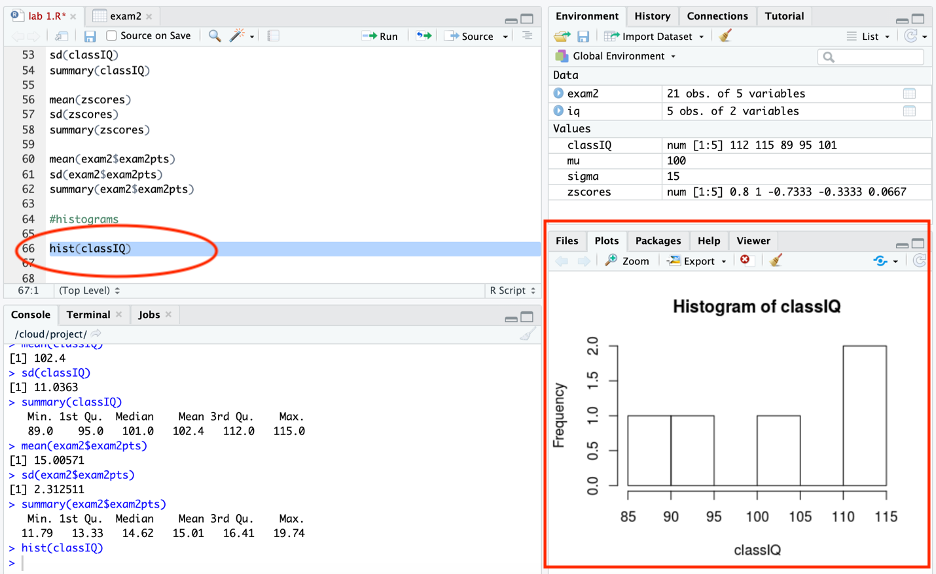
\includegraphics{img/basehist.png}
I circled and boxed what should match here. (Please excuse a few differences between this screenshot and your screen, like the name of the script, the code in the script before the histogram, and the results in the console. I had presented the material in a different order the last time I taught it.)

In order to use a base R function with a variable within a data frame you have to tell R to first look in the data frame in order to find the variable. You do this with the dollar sign (\texttt{\$}). Place the \texttt{\$} between the name of the data frame and the name of the variable.

For example, to use the \texttt{hist()} function to create a histogram of the exam 2 points variable in the exam 2 dataset, use this code:

\texttt{hist(exam2\$exam2pts)}\\
- exam2\$exam2pts is telling R to first go to the exam2 dataset and then use the exam2pts variable

Here is a picture:\\
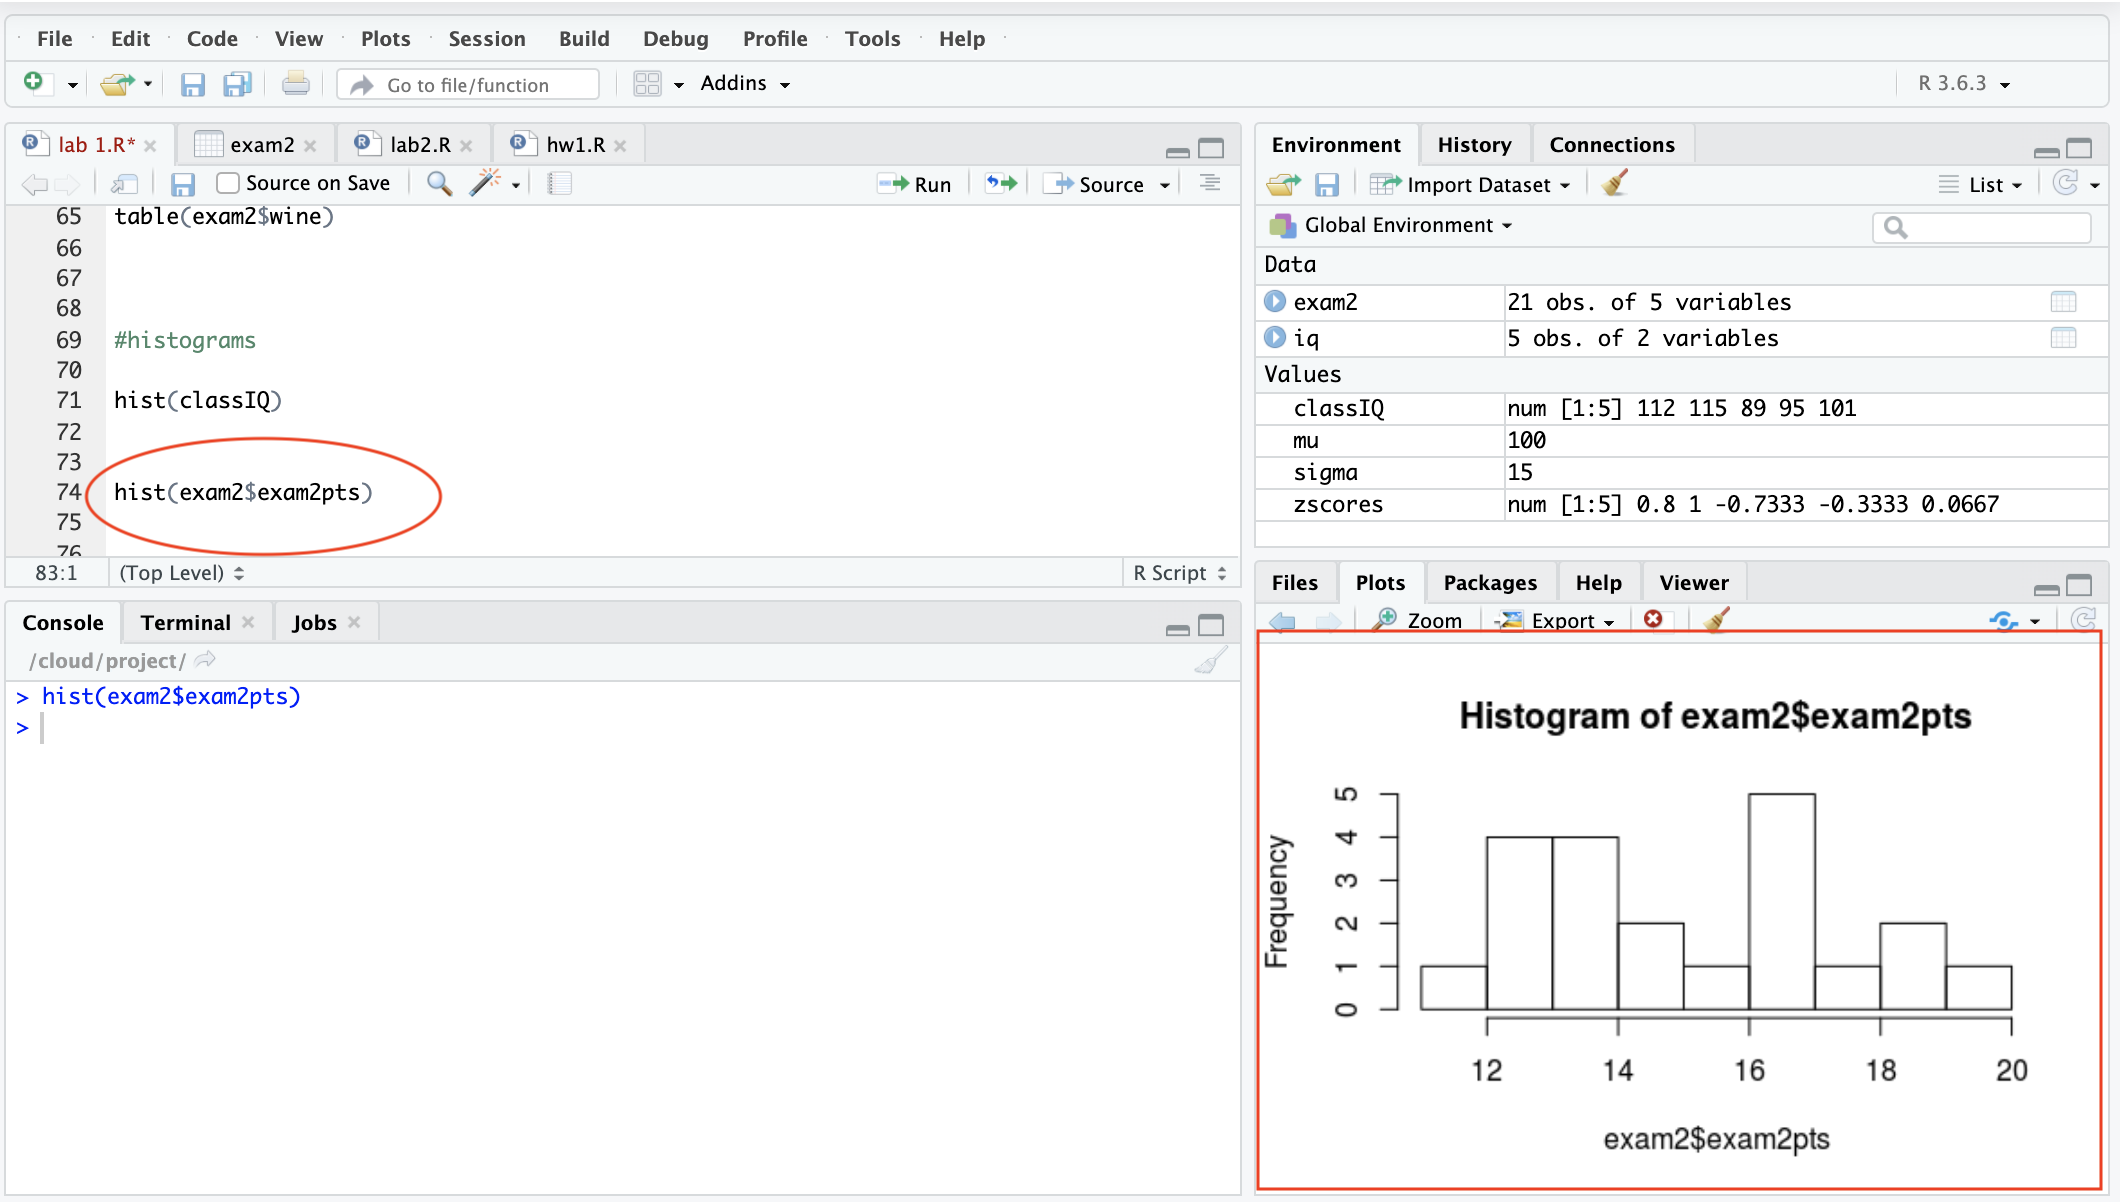
\includegraphics{img/basehist2.png}

The data looks some what normally distributed, with a slight positive shew.

\hypertarget{histograms-with-tidyverse}{%
\subsection{Histograms with tidyverse}\label{histograms-with-tidyverse}}

The base R option is quick and easy. But it is not customizable. Because of this -- many people prefer to use \textbf{ggplot} (of the Tidyverse package - so tidyverse needs to be loaded).

Ggplot is typically taught with the analogy of a globe that is built one layer at a time. You start with a world of only ocean (no land). Then you progressively add ``layers'' of land, colors, terrain, legends, etc. This system is based on the grammar of graphics: statistical graphics map \textbf{data} onto perceivable \textbf{aesthetic attributes} (e.g., position, color, shape, size, line type) of \textbf{geometric objects} (e.g., points, bars, lines). Code can also be added to ggplots to make graphs in APA style.

With ggplot, you build plots step-by-step, layer-by-layer using the following steps:\\
1. Start with \texttt{ggplot()}\\
2. Supply a dataset and aesthetic mapping, \texttt{aes()}\\
3. Add on \ldots{}\\
+ \textbf{Layers}, like \texttt{geom\_point()} or \texttt{geom\_histogram()}\\
+ \textbf{Scales}, like \texttt{scale\_colour\_brewer()}\\
+ \textbf{Faceting Specifications}, like \texttt{facet\_wrap()}\\
+ \textbf{Coordinate Systems}, like \texttt{coord\_flip()}

The code for a histogram of the exam 2 points is:\\
\texttt{ggplot(exam2,\ aes(x=exam2pts))\ +}~\\
\texttt{geom\_histogram(binwidth=1)}

\begin{itemize}
\tightlist
\item
  The first line starts with ggplot and then supplies a dataset and aesthetic mapping, \texttt{aes()}

  \begin{itemize}
  \tightlist
  \item
    Because you supply the dataset this way - you do not need to use \texttt{\$} to tell R where the variable is\\
  \end{itemize}
\item
  The second line adds the layer of a histogram
\end{itemize}

After you run this code your screen should look like this:

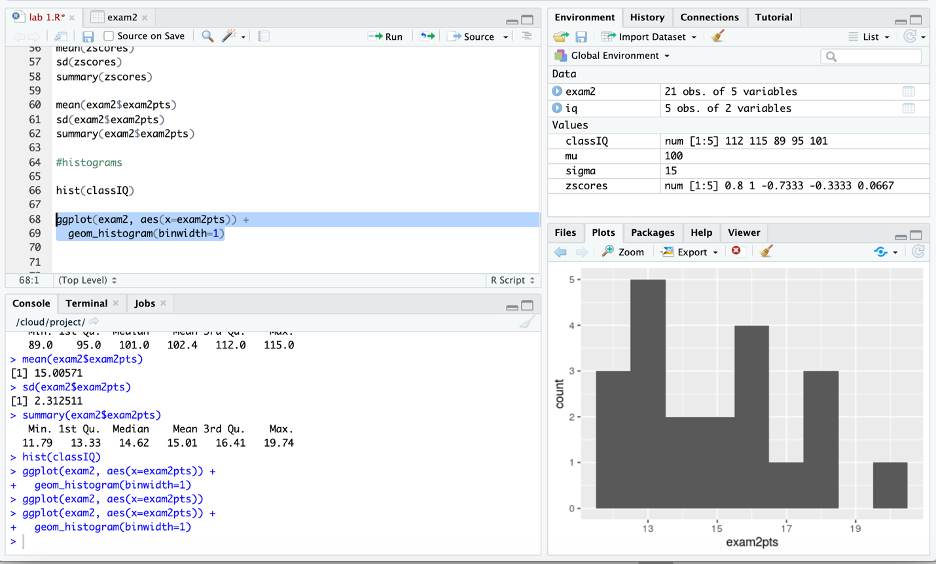
\includegraphics{img/tidyhist.png}

Note that the histogram here is more detailed than the one you produced with base R. This is because base R used 5-points bins, while ggplot used 1-point bins (because you told R to). Here it is easier to see that the data is slightly skewed right.

In ggplot, it is easy to change the amount of points per bin by changing the number after the binwidth. For example, here I change the number to 3:

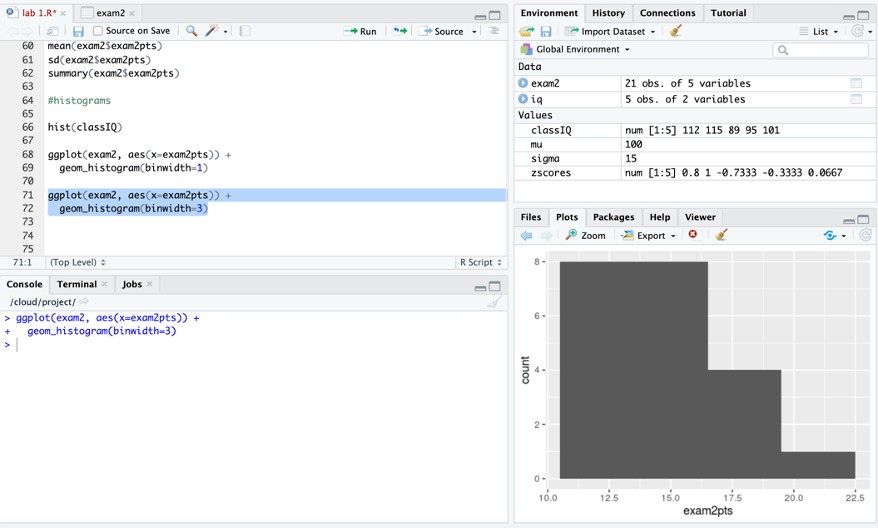
\includegraphics{img/tidyhist2.png}
Some say that 10 bins in a histogram is a good rule of thumb (There are more precise equations for determining the ``right'' number of bins as well).

Let's look at a histogram of the number of hours studied for exam 2 next.

Here is the code:

\texttt{ggplot(exam2,\ aes(x=hrsstudye2))\ +}\\
\texttt{geom\_histogram(binwidth=1)}

After you run this code, your screen should look like this:\\
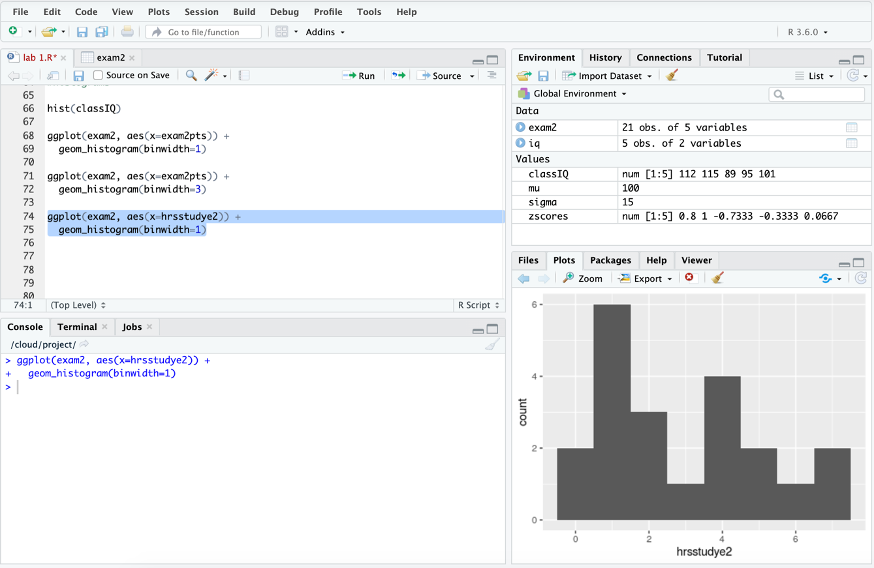
\includegraphics{img/tidyhist3.png}

The histogram show that data approximates the normal distribution and is roughly mound shape.

You do not need to run this -- but I just want to show you that if I run only the first line of the histogram code, the figure would look like this:

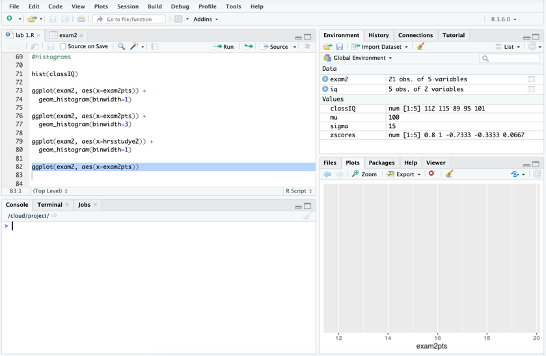
\includegraphics{img/ggoc.png}

\ldots so this is the world as only ocean -- without land. The second line of the ggplot code (i.e.~\texttt{geom\_histogram(binwidth=1})) adds the ``land''.

\emph{Please note that I am going to start providing less screen shots of the whole Rstudio window from this point forward. When I include R code know that I mean that the code should be typed into a script.}

\hypertarget{scatterplots}{%
\section{Scatterplots}\label{scatterplots}}

A \textbf{Scatterplot} is a graph where one variable is plotted on the y-axis and the other is plotted on the x-axis. Each dot represents one participant, measured on two variables.

We are going to focus on using ggplots to create scatterplots because it is the more powerful data visualization tool in R.

\hypertarget{two-continuous-variables}{%
\subsection{Two continuous variables}\label{two-continuous-variables}}

Using the exam 2 dataset, let's say we hypothesized that there is a positive association between exam 2 scores and the number of hours studied for the exam. One of the first steps of exploring this association is to create a scatterplot.

Here is the code and resulting graph:

\begin{Shaded}
\begin{Highlighting}[]
\KeywordTok{ggplot}\NormalTok{(exam2, }\KeywordTok{aes}\NormalTok{(}\DataTypeTok{x=}\NormalTok{exam2pts, }\DataTypeTok{y=}\NormalTok{hrsstudye2)) }\OperatorTok{+}
\StringTok{  }\KeywordTok{geom_point}\NormalTok{()}
\end{Highlighting}
\end{Shaded}

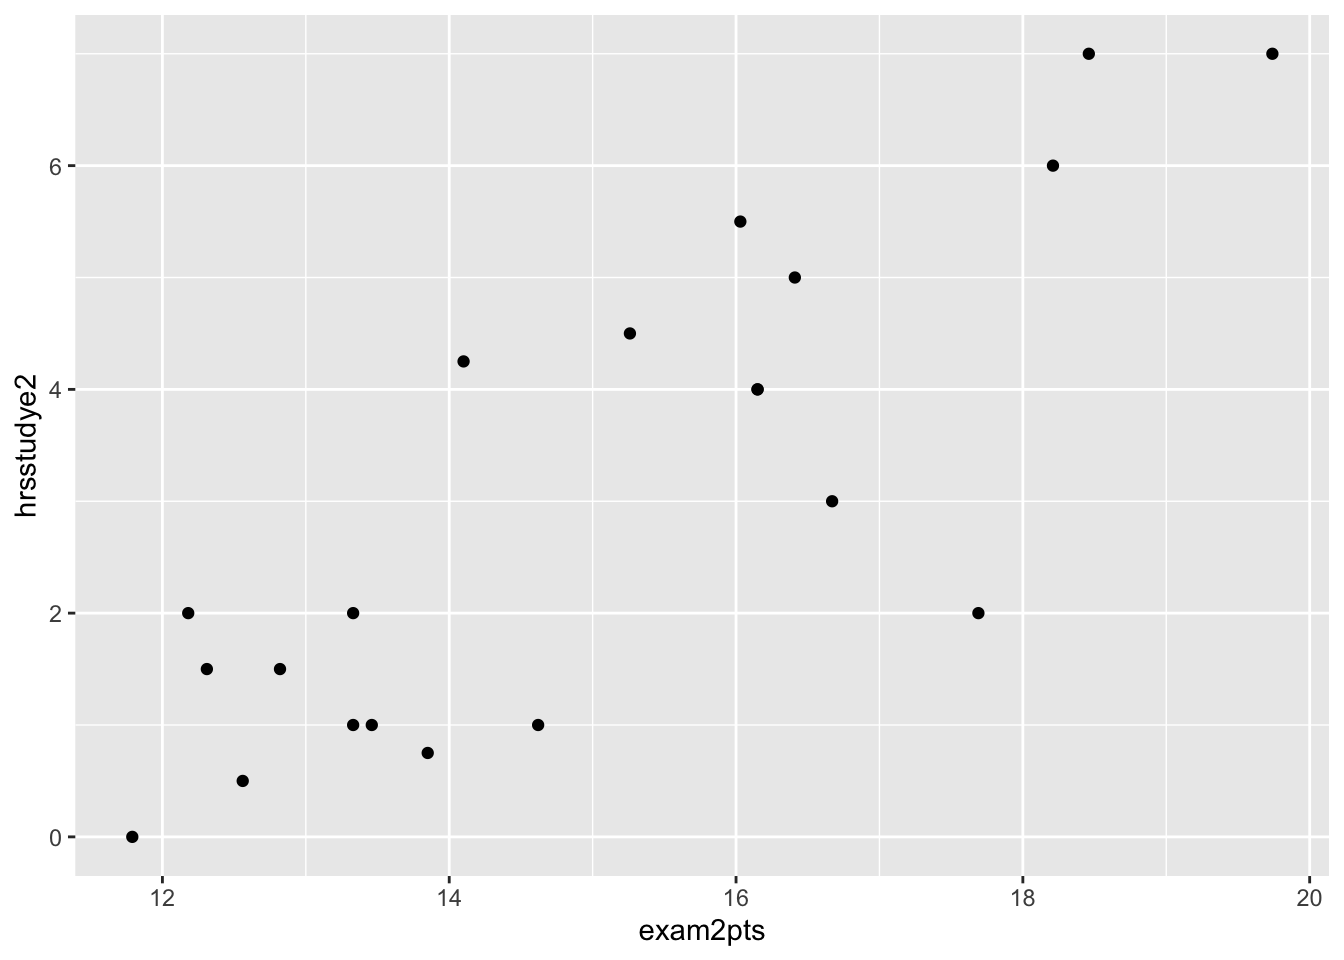
\includegraphics{Tools-for-working-with-data-327_files/figure-latex/unnamed-chunk-2-1.pdf}

The data points are trending upward, suggesting a positive relation between exam 2 scores and the number of hours. The students who studied longer for the exam received higher grades; While those students who studied for less time received lower grades.

\hypertarget{one-continuous-and-one-categorical-variable}{%
\subsection{One continuous and one categorical variable}\label{one-continuous-and-one-categorical-variable}}

Let's say you were interested in the relation between cheese eating and exam 2 scores. You hypothesized that exam scores will be lowers for students who ate cheese the night before the exam because cheese gives nightmares.

Traditionally psychology likes to visualize the relation between a continuous and categorical variable using a bar graph. However, bar graphs can be misleading about the true nature of the data. Because of this, I prefer to continue to use a scatterplot to look at the association between a continuous and categorical variable - with some alterations to show the mean and variability (which is important to show with group data).

In ggplots you can alter the scatterplot to include the mean and variability, in addition to the actual data points, by including the \texttt{stat\_summary()} function in the ggplot code. The \texttt{stat\_summary()} function adds statistics to a ggplot.

To use the \texttt{stat\_summary()} function you need to install the Hmisc package. It does not need to be loaded. \emph{This is a rare exception on how packages in R normally work - The package does not need to be loaded in order for R to use it.}

Here is the code to install Hmisc:

\texttt{install.packages("Hmisc")}\\
- remember to be patient and wait until the package is completely installed.

Then create the scatterplot with the following ggplot code:

\texttt{ggplot(exam2,\ aes(x\ =\ cheese,\ y\ =\ exam2pts))\ +}\\
\texttt{geom\_point()\ +}~\\
\texttt{stat\_summary(fun.data\ =\ mean\_cl\_normal)}

\begin{itemize}
\tightlist
\item
  x is the categorical variable\\
\item
  y is the continuous variable\\
\item
  \texttt{geom\_point()} includes the data points\\
\item
  The \texttt{fun.data\ =\ mean\_cl\_normal} within the \texttt{stat\_summary()} function adds the mean and the confidence interval around the mean.
\end{itemize}

The graph should look like this:

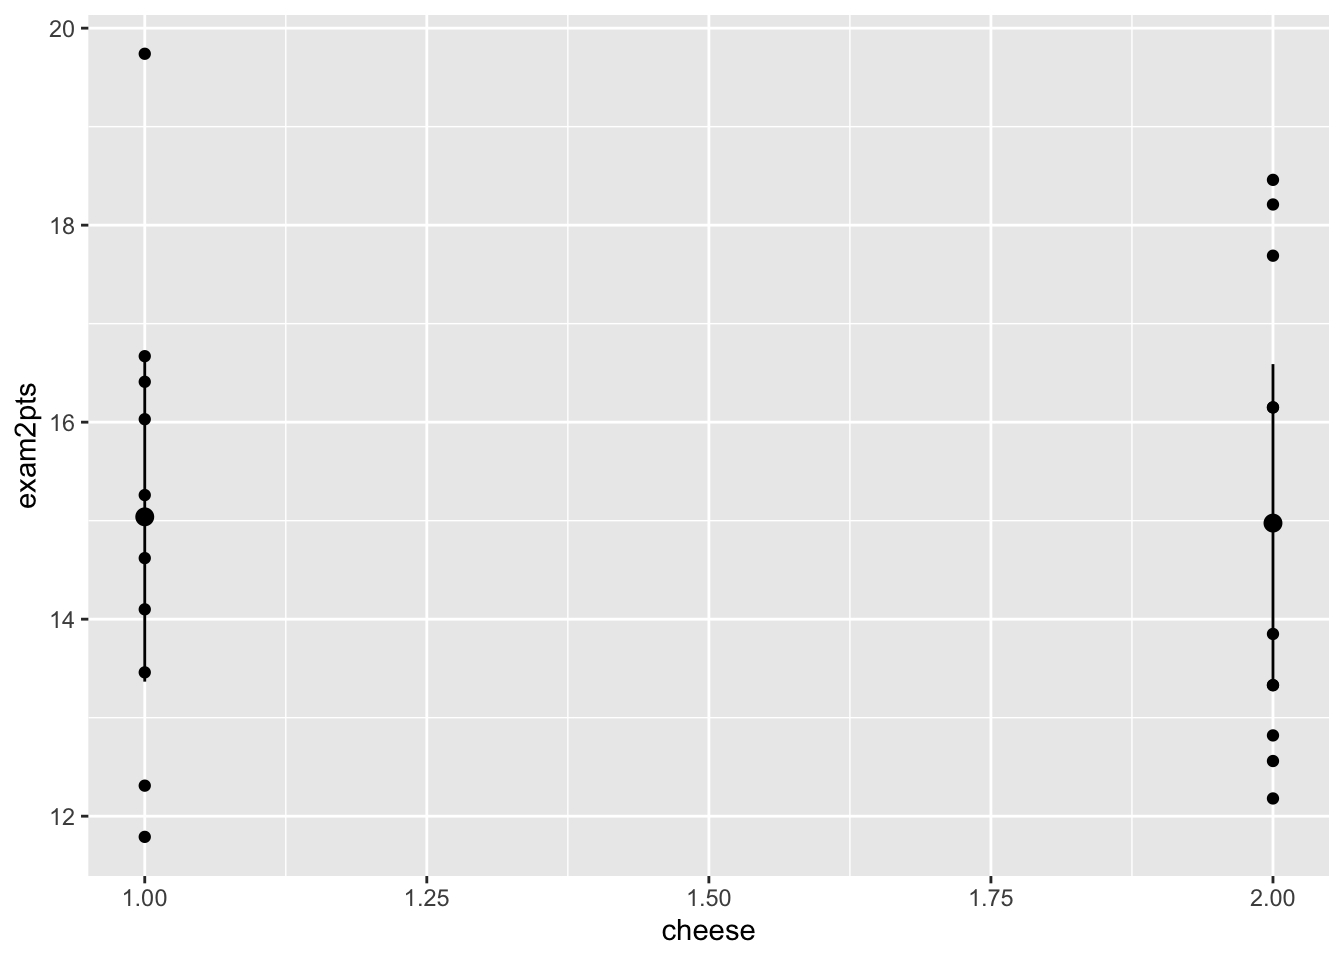
\includegraphics{Tools-for-working-with-data-327_files/figure-latex/unnamed-chunk-3-1.pdf}

The means are represented by the large dots. The lines represent the 95\% confidence intervals, which shows the certainty around the mean and is based on the sample mean, standard deviation, and n.~

The small dots are the data points representing the participants cheese eating and exam grades.

Here you can see that the mean exam 2 scores are pretty similar for students who did and did not eat cheese the night before the exam. The spread of the scores is also similar. (Remember from the introduction chapter 1 = no and 2 = yes).

I like to make a few alterations to the previous code for aesthetics\ldots{}

\texttt{ggplot(exam2,\ aes(x\ =\ as.factor(cheese),\ y\ =\ exam2pts))\ +}\\
\texttt{geom\_point(color\ =\ "purple")\ +}~\\
\texttt{stat\_summary(fun.data\ =\ mean\_cl\_normal)}

\begin{itemize}
\tightlist
\item
  The \texttt{color\ =\ "purple"} in the \texttt{geom\_point()} function changes the color of the data points making the graph easier to read\\
\item
  The \texttt{as.factor(cheese)} tells R to treat the cheese variable as a factor, which makes the x-axis more visually appealing
\end{itemize}

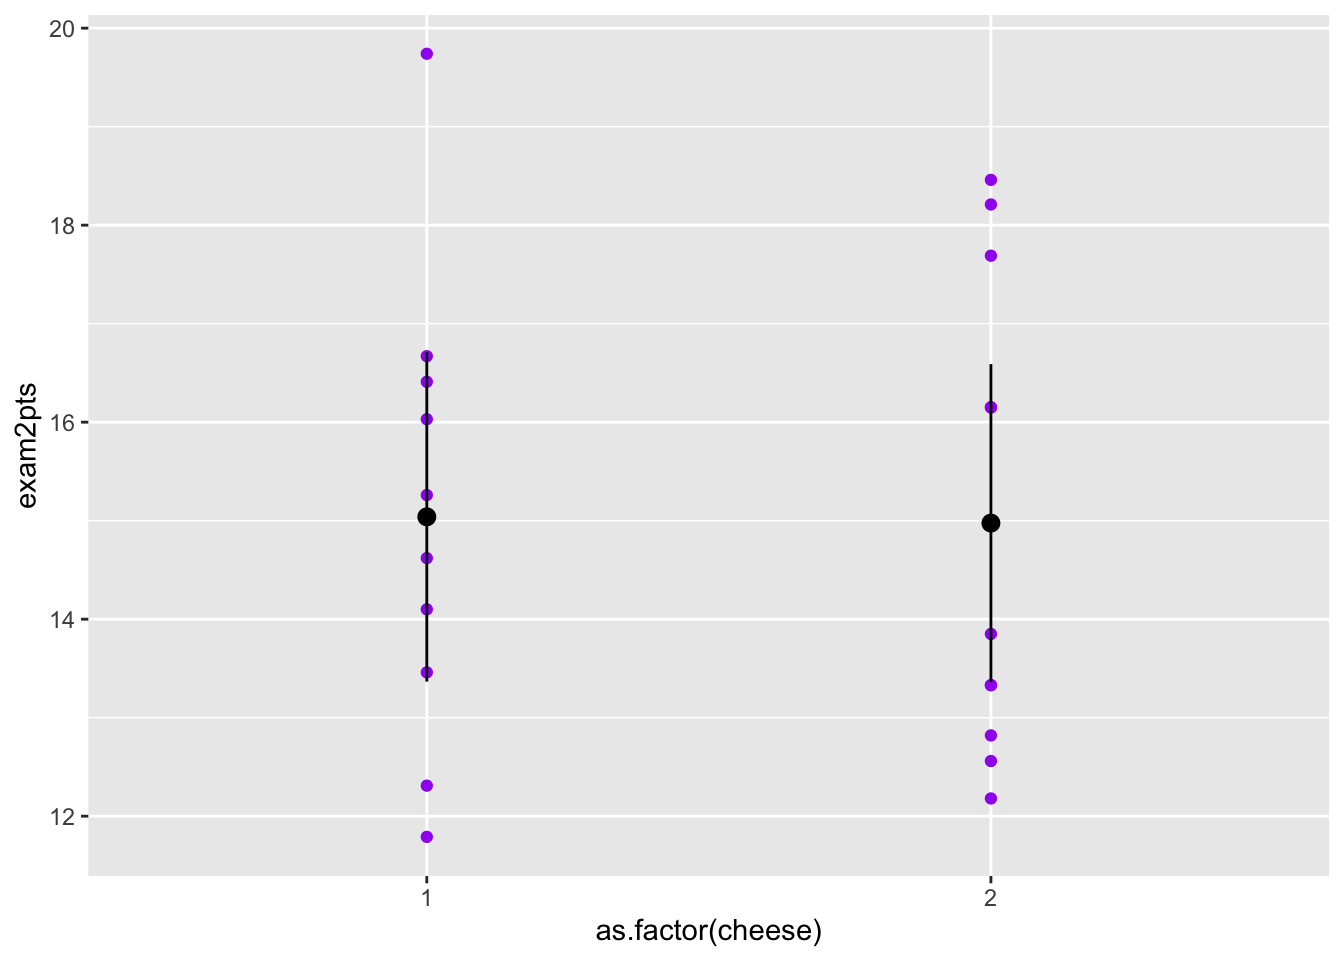
\includegraphics{Tools-for-working-with-data-327_files/figure-latex/unnamed-chunk-4-1.pdf}

\hypertarget{additional-resources}{%
\section{Additional resources}\label{additional-resources}}

\url{https://rstudio.cloud/learn/primers/1.1}

\hypertarget{descriptive-statistics}{%
\chapter{Descriptive Statistics}\label{descriptive-statistics}}

\textbf{NOTE:} Please open a new script and save it as lab 3 (or week 3) for your reproduction of this chapter.

This section focuses on functions that find descriptive statistics. \textbf{Descriptive statistics} refer to measures of central tendency (mean, median, and mode) and measures of variability (standard deviation, variance, range, etc.).

There are several functions that find descriptive statistics within R. My preferred method uses the Tidyverse and Psych packages, which I describe first. Next I will show you how to find descriptive statistics using base R.

\hypertarget{descriptive-statistics-using-tidyverse-and-psych-packages.}{%
\section{Descriptive statistics using Tidyverse and Psych packages.}\label{descriptive-statistics-using-tidyverse-and-psych-packages.}}

First load the tidyverse and psych packages (if they are not already loaded)

\begin{Shaded}
\begin{Highlighting}[]
\KeywordTok{library}\NormalTok{(tidyverse)}
\KeywordTok{library}\NormalTok{(psych)}
\end{Highlighting}
\end{Shaded}

The \texttt{describe()} function of the Psych package was made to produce the most frequently requested stats in psychology research in an easy to read data frame. I pair this with tidyverse styled code (because of the piping - which I explain next).

Here is the code to get descriptive statistics for the exam2 dataset we made:

\texttt{exam2\ \%\textgreater{}\%}\\
\texttt{describe()}

\begin{itemize}
\tightlist
\item
  The \texttt{describe()} function applies to all of the variables in the dataset (here exam2)
\item
  The \texttt{\%\textgreater{}\%} in this code is called a \textbf{pipe}
\item
  Pipes are part of the Tidyverse package
\item
  The shortcut to write a pipe (\texttt{\%\textgreater{}\%}) is \texttt{shift\ +\ command\ +\ M\ (shift\ +\ alt\ +\ M\ on\ a\ pc)}
\item
  Pipes are a way to write strings of functions more easily
\item
  You can think of it as a ``THEN''
\item
  So this code would be read as ``use the exam2 dataset'' THEN ``compute descriptive statistics with the describe function''
\end{itemize}

The twitter handle WeAreRladies uses this example to show the sequential nature of a pipe ( \%\textgreater\% ):\\
I woke up \%\textgreater\% showered \%\textgreater\% dressed \%\textgreater\% glammed up \%\textgreater\% took breakfast \%\textgreater\% showed up to work

Let's look at the results

\begin{verbatim}
##            vars  n  mean   sd median trimmed  mad   min   max range  skew
## id            1 21 11.00 6.20  11.00   11.00 7.41  1.00 21.00 20.00  0.00
## exam2pts      2 21 15.01 2.31  14.62   14.88 2.65 11.79 19.74  7.95  0.37
## hrsstudye2    3 21  3.02 2.20   2.00    2.88 2.22  0.00  7.00  7.00  0.41
## cheese        4 21  1.52 0.51   2.00    1.53 0.00  1.00  2.00  1.00 -0.09
## wine          5 21  1.48 0.51   1.00    1.47 0.00  1.00  2.00  1.00  0.09
##            kurtosis   se
## id            -1.37 1.35
## exam2pts      -1.13 0.50
## hrsstudye2    -1.26 0.48
## cheese        -2.08 0.11
## wine          -2.08 0.11
\end{verbatim}

The results show that the average exam points was 15.01 (out of 20), with a standard deviation of 2.31 points. Students studied for the exam for an average of 3.02 hours (SD = 2.20).

As the cheese and wine variables are nominal, the mean and standard deviation are not particularly meaningful. Also, any statistics on the ID numbers are meaningless.

This is a good place to mention that it is vital that you as a researcher understand what the numbers you are looking at are and the assumptions that they carry. R (or any computer program) will not tell you if what you asked for does not make sense or is not appropriate.

Rather than getting meaningless results that you have to ignore, you could add the \texttt{select()} function to the command above to select certain variables within a dataset. Note that you must include more than one variable for the \texttt{select()} function. Use the \texttt{pull()} function if you want to select only one variable.

For example, to select the exam2pts and hrsstudye2 variables use the following code:

\begin{Shaded}
\begin{Highlighting}[]
\NormalTok{exam2 }\OperatorTok
\StringTok{  }\KeywordTok{select}\NormalTok{(exam2pts, hrsstudye2) }\OperatorTok\StringTok{ }
\StringTok{  }\KeywordTok{describe}\NormalTok{()}
\end{Highlighting}
\end{Shaded}

\begin{verbatim}
##            vars  n  mean   sd median trimmed  mad   min   max range skew
## exam2pts      1 21 15.01 2.31  14.62   14.88 2.65 11.79 19.74  7.95 0.37
## hrsstudye2    2 21  3.02 2.20   2.00    2.88 2.22  0.00  7.00  7.00 0.41
##            kurtosis   se
## exam2pts      -1.13 0.50
## hrsstudye2    -1.26 0.48
\end{verbatim}

You should create frequency tables for nominal data. Do this with the \texttt{count()} function.

For example, create a frequency table for the cheese variable with this code:

\begin{Shaded}
\begin{Highlighting}[]
\NormalTok{exam2 }\OperatorTok\StringTok{ }
\StringTok{  }\KeywordTok{count}\NormalTok{(cheese)}
\end{Highlighting}
\end{Shaded}

\begin{verbatim}
## # A tibble: 2 x 2
##   cheese     n
##    <dbl> <int>
## 1      1    10
## 2      2    11
\end{verbatim}

\begin{itemize}
\tightlist
\item
  this code is saying to "use the exam 2 dataset and then count the cheese varible.
\end{itemize}

The results show that 10 students did not eat cheese the night before Exam 2 (see Introduction for codebook -- or what the 1 and 2 mean) and 11 students did eat cheese the night before the exam.

Finally, often we want to know descriptive statistics by group. For example, say you were interested in relation between cheese eating and exam 2 scores. You would want to know the descriptive statistics of the exam 2 scores for the students who did and did not eat cheese.

To do this I use the \texttt{describeBy()} function of the psych package, which reports basic summary statistics by a grouping variable. You have to tell R where to find the grouping variable by first including the dataset, followed by a \texttt{\$} and the variable name. In this example: \texttt{exam2\$cheese} (I can't figure out how to avoid the \texttt{\$} here - I will give extra credit if you can.)

Use the \texttt{pull()} function to select the exam2pts variable.

\begin{Shaded}
\begin{Highlighting}[]
\NormalTok{exam2 }\OperatorTok
\StringTok{  }\KeywordTok{pull}\NormalTok{(exam2pts) }\OperatorTok\StringTok{ }
\StringTok{  }\KeywordTok{describeBy}\NormalTok{(exam2}\OperatorTok{$}\NormalTok{cheese)}
\end{Highlighting}
\end{Shaded}

\begin{verbatim}
## 
##  Descriptive statistics by group 
## group: 1
##    vars  n  mean   sd median trimmed  mad   min   max range skew kurtosis   se
## X1    1 10 15.04 2.34  14.94   14.86 2.19 11.79 19.74  7.95 0.41    -0.75 0.74
## ------------------------------------------------------------ 
## group: 2
##    vars  n  mean  sd median trimmed  mad   min   max range skew kurtosis   se
## X1    1 11 14.98 2.4  13.85    14.9 2.48 12.18 18.46  6.28 0.28    -1.78 0.72
\end{verbatim}

The results show that the average exam 2 score for students who ate cheese was 15.05 (SD = 2.34) and the average exam 2 score for students who did not ate cheese was 14.98 (SD = 2.4). Other statistics that you might find useful are the group's n, median, minimum and maximum scores, range, and standard error (se).

\hypertarget{descriptive-statistics-using-base-r}{%
\section{Descriptive statistics using base R}\label{descriptive-statistics-using-base-r}}

Descriptive statistics can also be computed using base R.

When a variable is stored directly in an object, you can apply the mean and standard deviation functions to the object.

For example:

\begin{Shaded}
\begin{Highlighting}[]
\KeywordTok{mean}\NormalTok{(classIQ)}
\end{Highlighting}
\end{Shaded}

\begin{verbatim}
## [1] 102.4
\end{verbatim}

\begin{Shaded}
\begin{Highlighting}[]
\KeywordTok{sd}\NormalTok{(classIQ)}
\end{Highlighting}
\end{Shaded}

\begin{verbatim}
## [1] 11.0363
\end{verbatim}

The summary function provides the range and median as well:

\begin{Shaded}
\begin{Highlighting}[]
\KeywordTok{summary}\NormalTok{(classIQ)}
\end{Highlighting}
\end{Shaded}

\begin{verbatim}
##    Min. 1st Qu.  Median    Mean 3rd Qu.    Max. 
##    89.0    95.0   101.0   102.4   112.0   115.0
\end{verbatim}

Remember that if a variable is in a data frame, you have to tell R to first look in the data frame in order to find the variable. You do this with the dollar sign (\texttt{\$}). Place the \texttt{\$} between the name of the data frame and the name of the variable.

For example, to find the average points earned on Exam 2 use the following code:

\begin{Shaded}
\begin{Highlighting}[]
\KeywordTok{mean}\NormalTok{(exam2}\OperatorTok{$}\NormalTok{exam2pts)}
\end{Highlighting}
\end{Shaded}

\begin{verbatim}
## [1] 15.00571
\end{verbatim}

Note that when typing this code RStudio will provide a list of the variables in the exam2 after you type the \texttt{\$}. It is very convenient.

The \texttt{table()} function of base R performs categorical tabulations of data, frequency tables, and cross tabulations.

For the present example, the code is:

\begin{Shaded}
\begin{Highlighting}[]
\KeywordTok{table}\NormalTok{(exam2}\OperatorTok{$}\NormalTok{cheese)}
\end{Highlighting}
\end{Shaded}

\begin{verbatim}
## 
##  1  2 
## 10 11
\end{verbatim}

Note that the table is laid out differently than the Tidyverse one above. But you can still easily see that 10 students did not eat cheese the night before Exam 2 and 11 students did eat cheese the night before the exam.

\emph{Some people think that the Tidyverse and Psych packages make computing descriptive statistics a bit easier/more direct/better/easier to understand than base R. You should decide which you prefer. (I tend to prefer Tidyverse and Psych). Another packages that compute descriptive statistics is skimr }

  \bibliography{book.bib,packages.bib}

\end{document}
